\documentclass[10pt,letterpaper,twocolumn]{article}
\usepackage{enumerate}
\usepackage{times}
\usepackage{epsfig}
\usepackage{graphicx}
\usepackage{setspace}
%\usepackage{amsmath}
\usepackage{amssymb}
%\usepackage{subfigure}
\usepackage{multirow}
%\usepackage[linesnumbered,noend,ruled]{algorithm2e}
\usepackage{float}
\usepackage{verbatim}
\usepackage[margin=0.5in]{geometry}
\usepackage[symbol]{footmisc}
\usepackage{courier}
%\usepackage[breaklinks=true,colorlinks,bookmarks=false]{hyperref}
\usepackage{caption}
\captionsetup{font=scriptsize}
\usepackage[export]{adjustbox}
\usepackage{fancybox}
\usepackage{authblk}
\usepackage{url}
\usepackage{latexsym}



%\DeclareCaptionFormat{myformat}{#1#2#3\hrulefill}
%\captionsetup{format=myformat}
\newcommand{\tab}{\hspace*{2em}}

\begin{document}

\title{Affine Loop Optimization Based On Modulo Unrolling in Chapel}
\author[1]{Aroon Sharma}
\author[1]{Darren Smith}
\author[1]{Joshua Koehler}
\author[1]{Rajeev Barua}
\author[2]{Michael Ferguson}
\affil[1]{Department of Electrical and Computer Engineering, University of Maryland College Park}
\affil[2]{Laboratory for Telecommunication Sciences, College Park, Maryland}

           
\maketitle

\begin{abstract}

This paper presents modulo unrolling without unrolling (WU), a method for message aggregation for parallel loops in message passing programs that use affine array accesses in Chapel, a Partitioned Global Address Space (PGAS) parallel programming language. Messages incur a non-trivial run time overhead, a significant component of which is independent of the size of the message. Therefore, aggregating messages improves performance. Our optimization for message aggregation is based on a technique known as modulo unrolling, pioneered by Barua \cite{barua1999maps}, whose purpose was to ensure a statically predictable single tile number for each memory reference for tiled architectures, such as the MIT Raw Machine \cite{waingold1997baring}. Modulo unrolling WU applies to data that is distributed in a cyclic or block-cyclic manner. In this paper, we adapt the aforementioned modulo unrolling technique to the difficult problem of efficiently compiling PGAS languages to message passing architectures. When applied to loops and data distributed cyclically or block-cyclically, modulo unrolling WU can decide when to aggregate messages thereby reducing the overall message count and runtime for a particular loop. Compared to other methods, modulo unrolling WU greatly simplifies the complex problem of automatic code generation of message passing code. It also results in substantial performance improvement compared to the non-optimized Chapel compiler. 

\begin{comment}
This paper presents a loop optimization for message passing programs that use affine array accesses in Chapel, a Partitioned Global Address Space (PGAS) parallel programming language. Each message in Chapel incurs some non-trivial run time overhead. Therefore, aggregating messages improves performance. The optimization is based on a technique known as modulo unrolling, where the locality of any affine array access can be deduced at compile time if the data is distributed in a cyclic or block cyclic fashion. First pioneered by Barua \cite{barua1999maps} for tiled architectures, we adapt modulo unrolling to the problem of compiling PGAS languages to message passing architectures. When applied to loops and data distributed cyclically or block cyclically, modulo unrolling can decide when to aggregate messages thereby reducing the overall message count and run time for a particular loop. Compared to other methods, modulo unrolling greatly simplifies the very complex problem of automatic code generation of message passing code from a PGAS language such as Chapel. It also results in substantial performance improvement compared to the non-optimized Chapel compiler.
\end{comment}

To implement this optimization in Chapel, we modify the leader and follower iterators in the Cyclic and Block Cyclic data distribution modules. Results were collected that compare the performance of Chapel programs optimized with modulo unrolling WU and Chapel programs using the existing Chapel data distributions. Data collected on a ten-locale cluster show that on average, modulo unrolling WU used with Chapel's Cyclic distribution results in 76 percent fewer messages and a 45 percent decrease in runtime for our suite of benchmarks. Similarly, modulo unrolling WU used with Chapel's Block Cyclic distribution results in 72 percent fewer messages and a 52 percent decrease in runtime. 

\end{abstract}



\section{Introduction}\label{sec:intro} 

Compilation of programs for distributed memory architectures using message passing is a vital task with potential for speedups over existing techniques. The partitioned global address space (PGAS) parallel programming model exposes locality of reference information to the programmer thereby improving programmability and allowing for compile-time performance optimizations. In particular, programs compiled to message passing hardware can improve in performance by aggregating messages and eliminating dynamic locality checks for affine array accesses in the PGAS model. 

Message passing code generation is a difficult task for an optimizing compiler targeting a distributed memory architecture. These architectures are comprised of independent units of computation called locales. Each locale has its own set of processors, cores, memory, and address space. For programs executed on these architectures, data is distributed across various locales of the system, and the compiler needs to reason about locality in order to determine whether a program data access is remote (requiring a message to another locale to request a data element) or local (requiring no message and accessing the data element on the locale's own memory). Only a compiler with sufficient knowledge about locality can compile a program in this way with good communication performance. 

Each remote data memory access results in a message with some non-trivial run time overhead, which can drastically slow down a program's execution time. This overhead is caused by latency on the interconnection network and locality checks for each data element. Accessing multiple remote data elements individually results in this run time overhead being incurred multiple times, whereas if they are transferred in bulk the overhead is only incurred once. Therefore, aggregating messages improves performance of message passing codes. In order to transfer remote data elements in bulk, the compiler must be sure that all elements in question are remote before the message is sent. 

The vast majority of loops in scientific programs access data using affine array accesses. An affine array access is a linear expression of the loop's index variables. Loops using affine array accesses are special because they exhibit regular access patterns within a data distribution. Compilers can use this information to decide when message aggregation can take place. 

Although a simple concept to understand, message aggregation is the most complicated part of message passing code generation. Existing methods \cite{goumas2006message, xue1997communication} split the loop iteration space into tiles (also known as footprints) of consecutive iterations, and each locale executes its tile's iterations in parallel. Communication using aggregation takes place between locales just before and after the computation within a single tile. These methods require the compiler to do complex footprint calculations, optimizing for tile size and shape, before message aggregation can take place. As \cite{ramanujam1992tiling} shows, determining tile shape quickly becomes difficult for more complicated loop structures, since the optimum tile shape for a computation is not always rectangular. It is our belief that message aggregation using tiling is not used in production quality compilers today because of the complexity of this footprint analysis. What is needed is a simple, robust, and widely applicable method for message aggregation that leads to improvements in performance. 

This paper presents a loop optimization for message passing code generation based on a technique called modulo unrolling, where the locality of any affine array access can be deduced at compile time if the data is distributed in a cyclic or block cyclic fashion. The optimization can be performed by a compiler to aggregate messages and reduce a program's execution time and communication. Modulo unrolling in its original form, pioneered by \cite{barua1999maps}, was meant to target tiled architectures such as the MIT Raw machine, not distributed memory architectures that use message passing. It has since been modified to apply to such machines in this work. In this work, modulo unrolling unrolls an affine loop by a factor equal to the number of locales of the machine being utilized by the program. If the arrays used in the loop are distributed cyclically or block cyclically, each array access is guaranteed reside on a single locale across all iterations of the loop. Using this information, the compiler can then aggregate all remote array accesses that reside on a remote locale into a single message before the loop. If remote array elements are written to during the loop, one message is required to store these elements back to each remote locale after the loop runs. 

Chapel is an explicitly parallel programming language developed by Cray Inc. that falls under the Partitioned Global Address Space (PGAS) memory model. Here, a system's memory is abstracted to a single global address space regardless of the hardware architecture and is then logically divided per locale and thread of execution. By doing so, locality of reference can easily be exploited no matter how the system architecture is organized. The Chapel compiler is an open source project used by many in industry and academic settings. The language contains many high level features such as zippered iteration and array slicing that greatly simplify the implementation of modulo unrolling into the language.

\subsection{Chapel's Data Distributions} 

In this work, we consider three types of data distributions: Block, Cyclic, and Block Cyclic. In a Block distribution, elements of an array are mapped to locales evenly in a dense manner. In a Cyclic distribution, elements of an array are mapped in a round-robin manner across locales. In a Block Cyclic distribution, a number of elements specified by a block size parameter is allocated to consecutive array indices in a round robin fashion. Figures \ref{block_dist} - \ref{cyc_dist} illustrate these three Chapel distributions for a two-dimensional array. In Figure \ref{block_cyc_dist}, the array takes a 2 x 2 block size parameter. 

The choice of data distribution to use for a program boils down to computation and communication efficiency. It has been shown that finding an optimal data distribution for parallel processing applications is an NP-complete problem, even for one or two dimensional arrays \cite{mace1987memory}. Certain program data access patterns will result in fewer communication calls if the data is distributed in a particular way. For example, many loops in stencil programs that contain nearest neighbor computation will have better communication performance if the data is distributed using a Block distribution. This occurs because on a given loop iteration, the elements accessed are near each other in the array and therefore more likely to reside on the same locale block. Accessing elements on the same block does not require a remote data access and can be done faster. However, programs that access array elements far away from each other will have better communication performance if data is distributed using a Cyclic distribution. Here, a Block distribution is almost guaranteed to have poor performance because the farther away accessed elements are the more likely they are to reside on different locales. 

A programmer may choose a particular data distribution for reasons unknown to the compiler. These reasons may not even take communication behavior into account. For example, Cyclic and Block Cyclic distributions provide better load balancing of data across locales than a Block distribution because elements can be added or removed according to a regular predictable pattern. In many applications, data redistribution may be needed if elements of a data set are inserted or deleted. In particular, algorithms to redistribute data using a new block size exist for the Block Cyclic distribution \cite{walker1996redistribution, prylli1997fast}. If an application uses a dynamic data set with elements being appended, a Cyclic or Block Cyclic distribution is superior to Block because new elements are added to the locale that follows the cyclic or block cyclic pattern. For Block, the entire data set would need to be redistributed every time a new element is appended, which can be expensive. 

Compatibility with other PGAS languages might be an important consideration for a programmer when selecting a data distribution. Data sets used by Chapel programs and other PGAS programs should use Cyclic or Block Cyclic distributions because other PGAS languages do not support the Block distribution. A programmer would benefit by distributing the same data set using only one scheme so the data would not have to be replicated for different programs. 

Therefore, in this work, it is our view that the compiler should not change the programmer's choice of data distribution in order to achieve better runtime and communication performance. The compiler should attempt to perform optimizations based on the data distribution that the programmer specified. 

\begin{figure}
	\begin{center}
	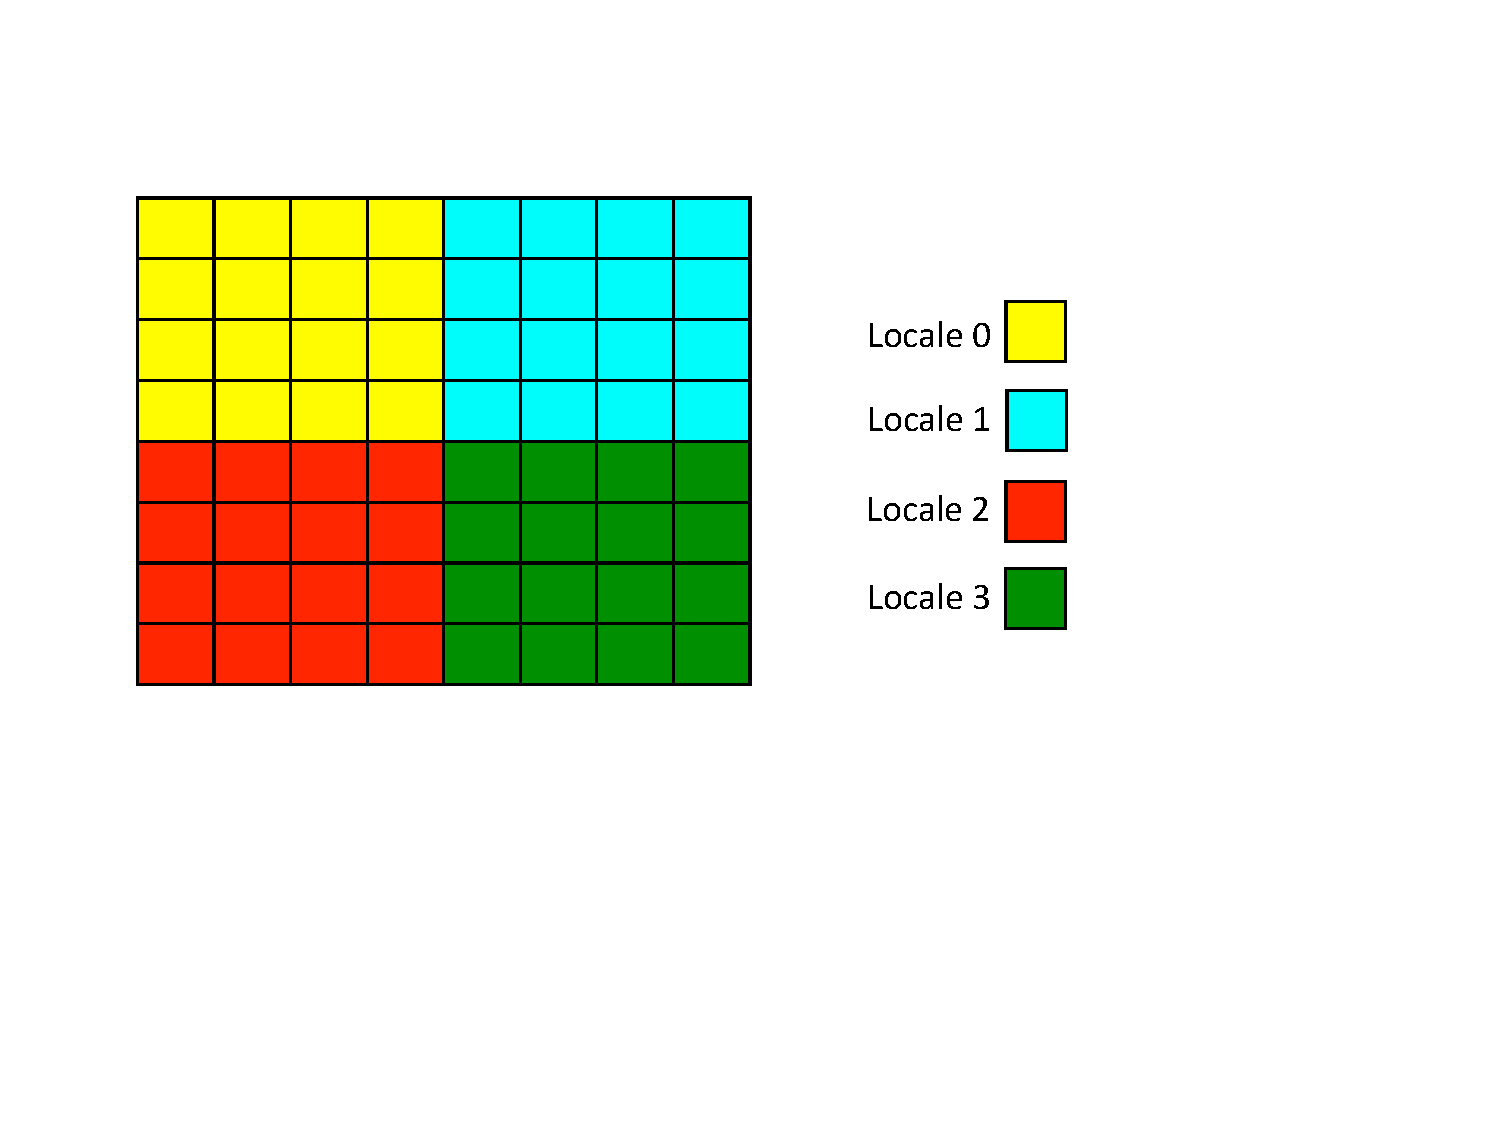
\includegraphics[scale=0.55]{./Figures/block_dist}
	\caption{Chapel Block distribution.}
	\label{block_dist}
	\end{center}
\end{figure}

\begin{figure}
	\begin{center}
	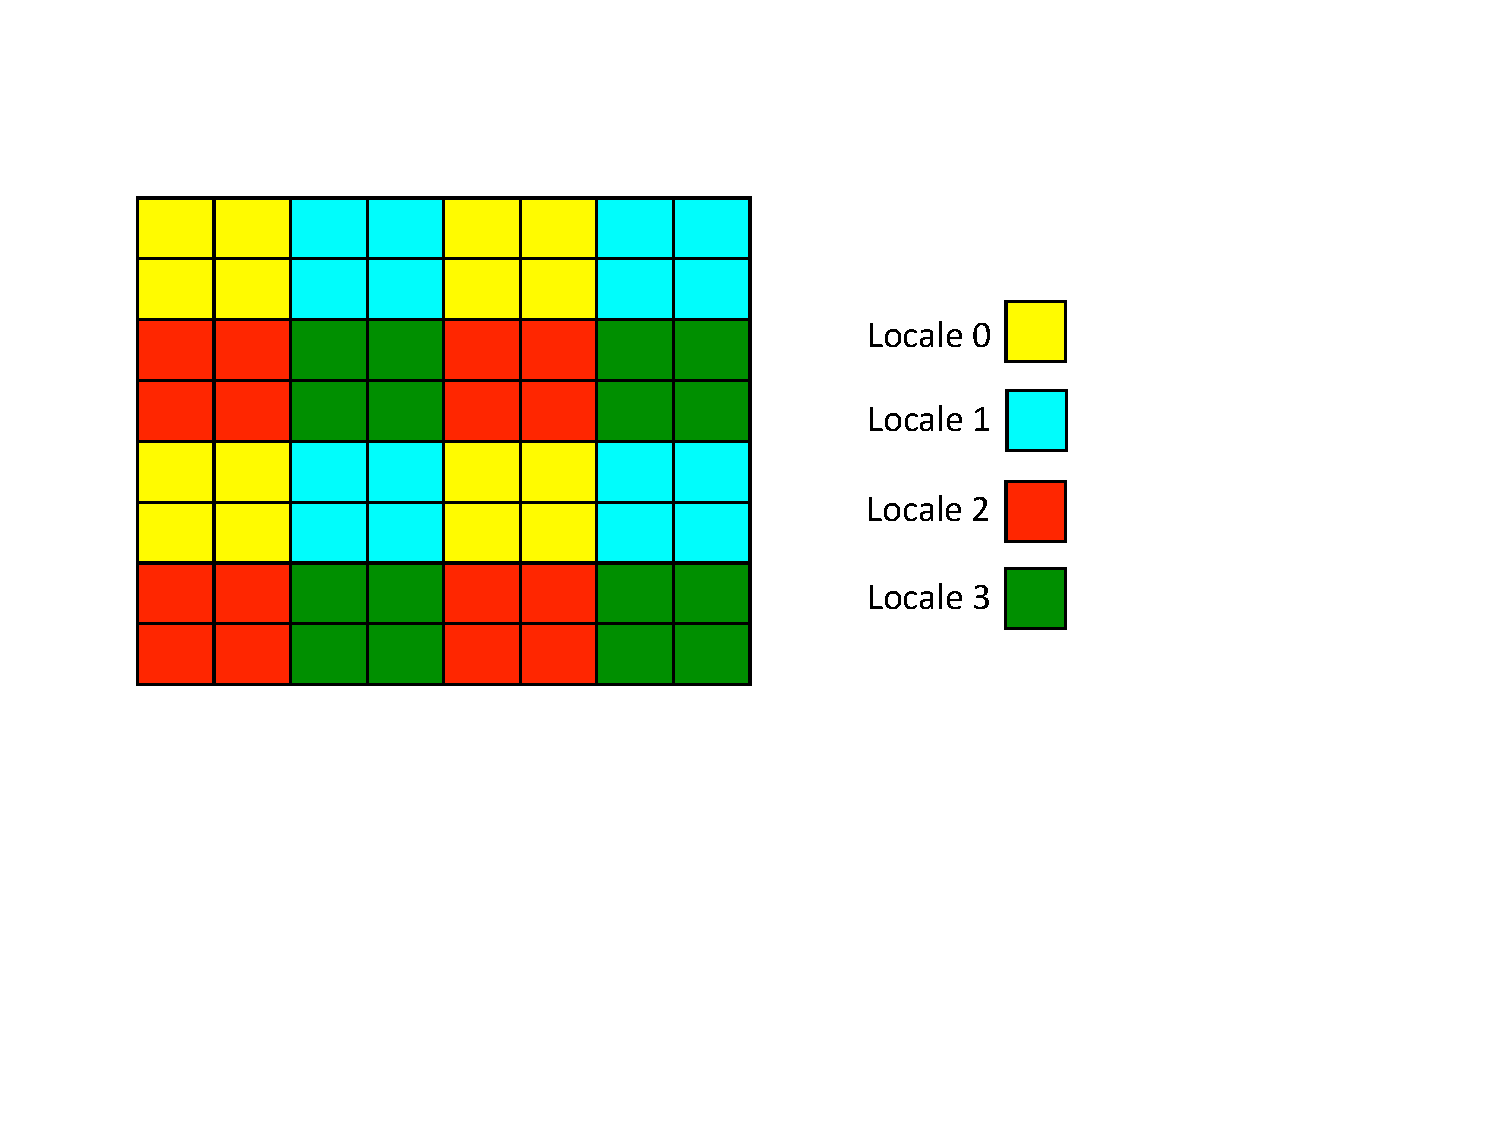
\includegraphics[scale=0.55]{./Figures/block_cyc_dist}
	\caption{Chapel Block Cyclic distribution with a 2 x 2 blocksize parameter.}
	\label{block_cyc_dist}
	\end{center}
\end{figure}

\begin{figure}
	\begin{center}
	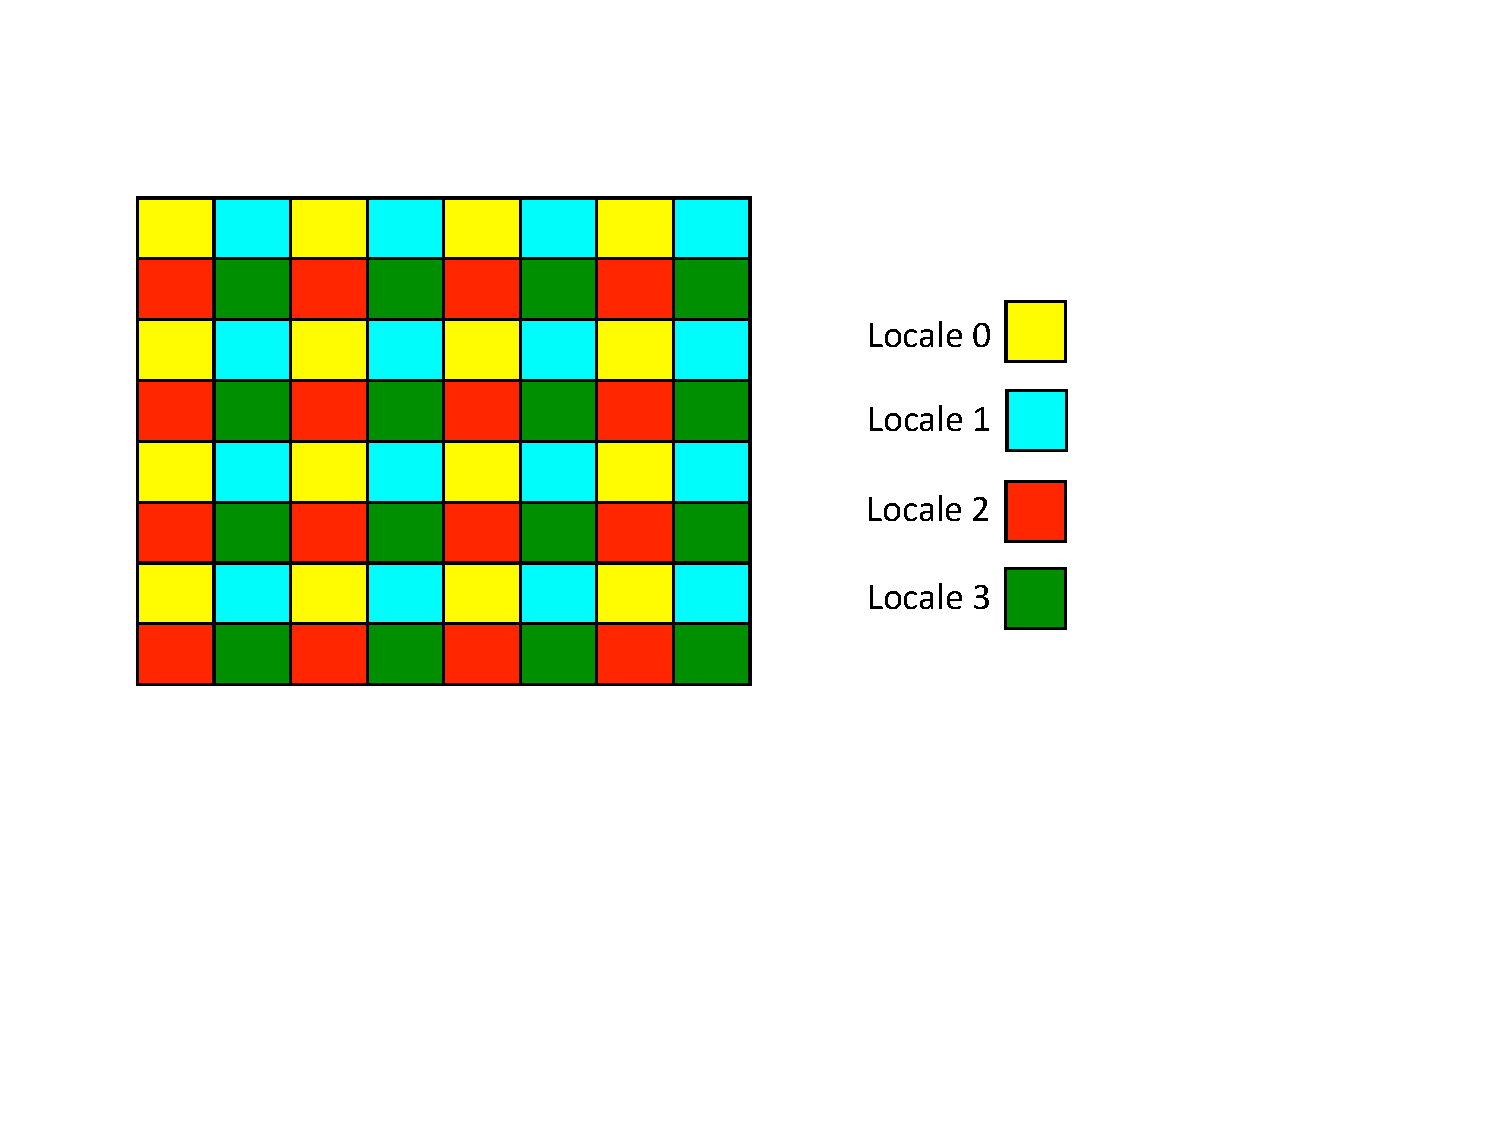
\includegraphics[scale=0.55]{./Figures/cyc_dist}
	\caption{Chapel Cyclic distribution.}
	\label{cyc_dist}
	\end{center}
\end{figure}




\section{Chapel's Data Distributions}\label{sec:data_distributions} 

Figures \ref{block_dist} - \ref{block_cyc_dist} illustrate the Chapel data distributions that we explored in this work: Block, Cyclic, and Block Cyclic. Each figure shows how a two-dimensional 8 x 8 array can be distributed in Chapel using each distribution. Figure \ref{block_dist} illustrates the Block distribution. Elements of the array are mapped to locales evenly in a dense manner. In Figure \ref{cyc_dist}, the Cyclic distribution, elements of the array are mapped in a round-robin manner across locales. Finally, in Figure \ref{block_cyc_dist} the Block Cyclic distribution is shown. Here, a number of elements specified by a block size parameter is allocated to consecutive array indices in a round-robin fashion. In Figure \ref{block_cyc_dist}, the distribution takes in a 2 x 2 block size parameter. Further details about Block, Cyclic, and Block Cyclic distributions in Chapel are described in \cite{distributions}.

\begin{figure}
\begin{center}
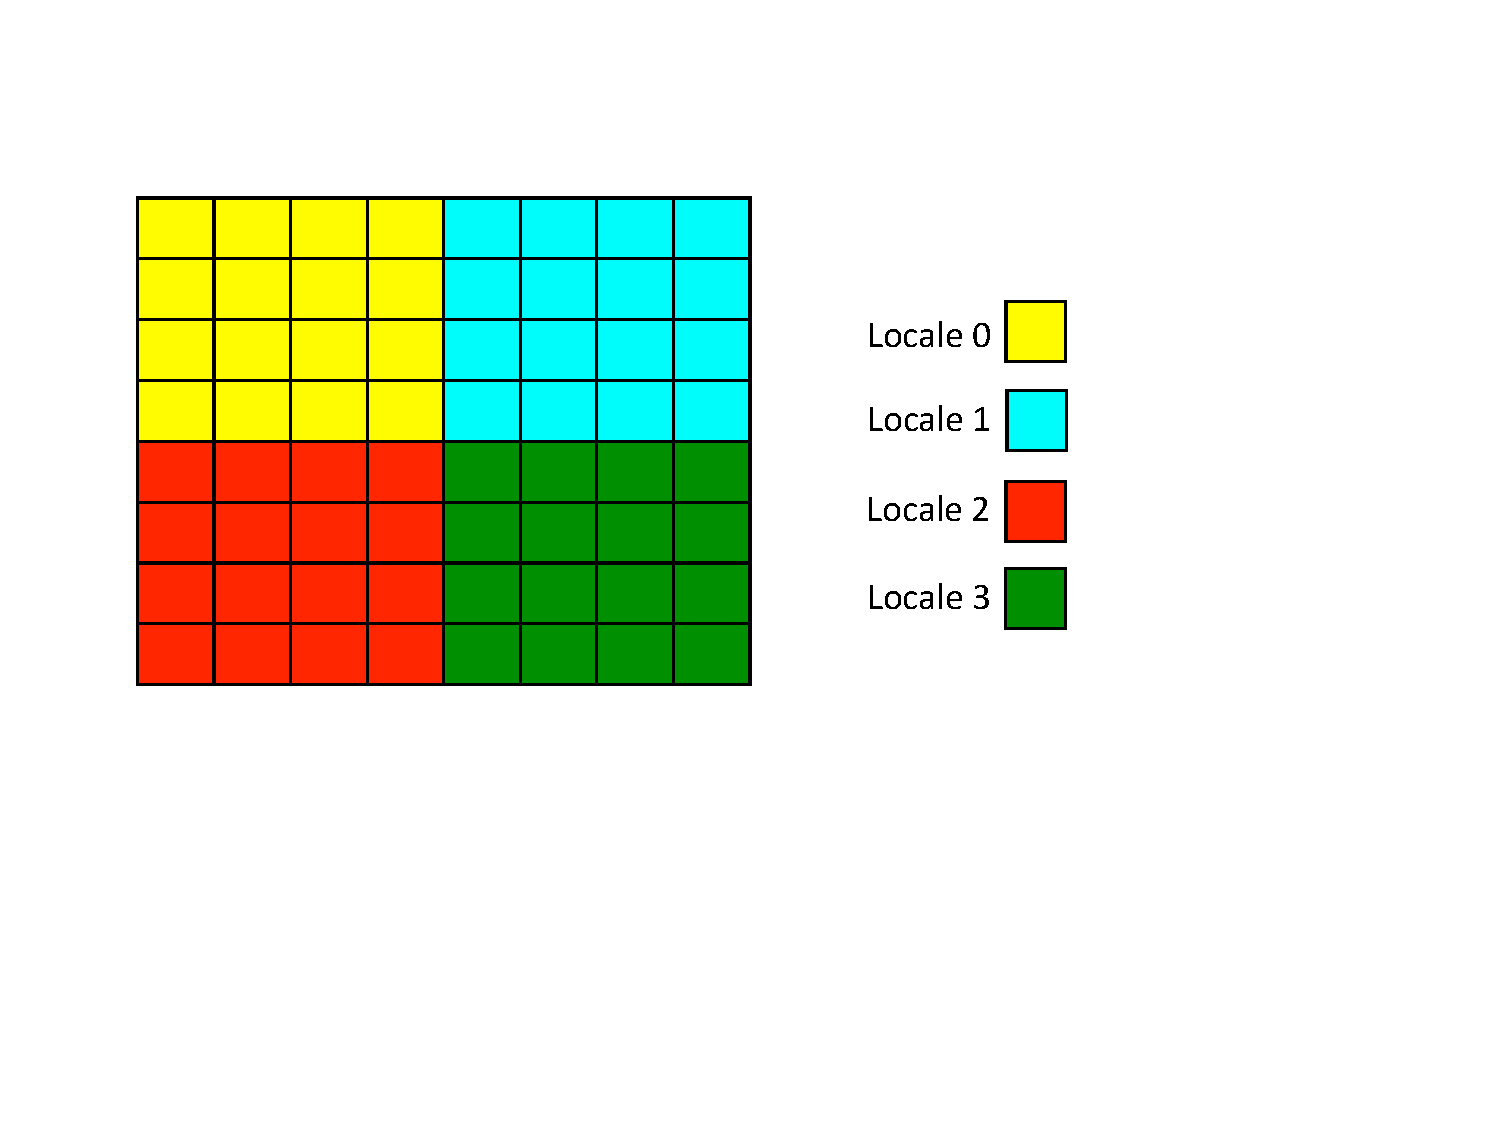
\includegraphics[width=\linewidth]{./Figures/block_dist}
\caption{Chapel Block distribution.}
\label{block_dist}
\end{center}
\end{figure}

\begin{figure}
\begin{center}
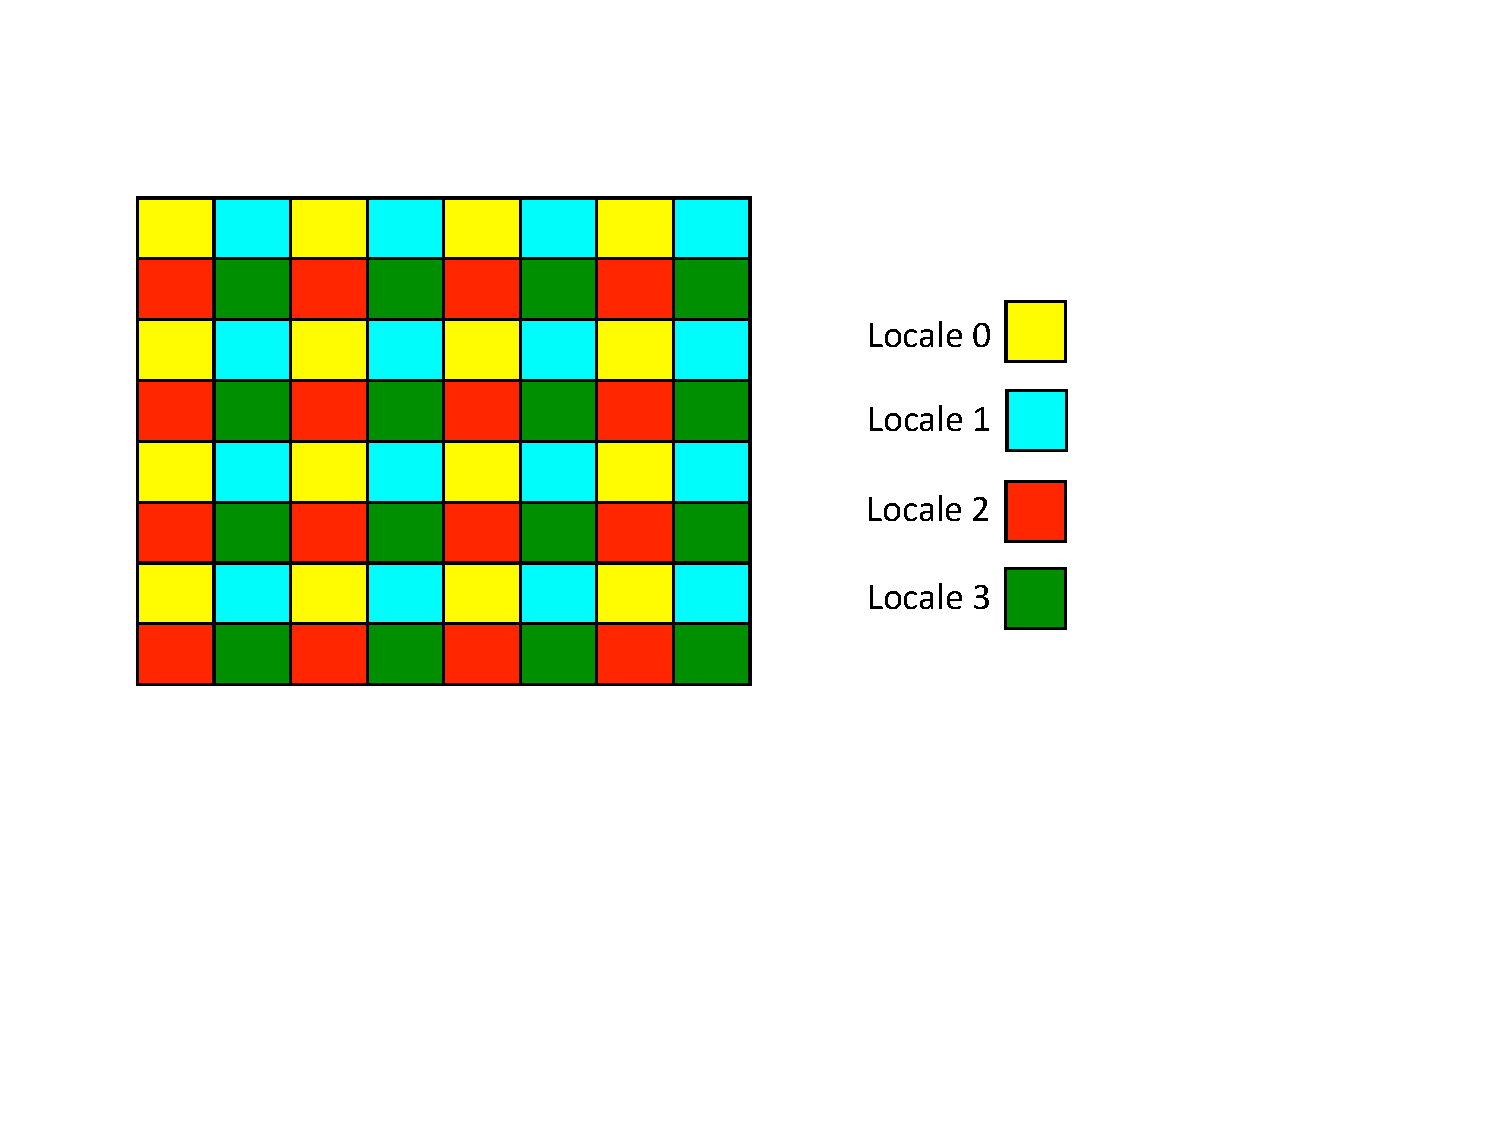
\includegraphics[width=\linewidth]{./Figures/cyc_dist}
\caption{Chapel Cyclic distribution.}
\label{cyc_dist}
\end{center}
\end{figure}

\begin{figure}
\begin{center}
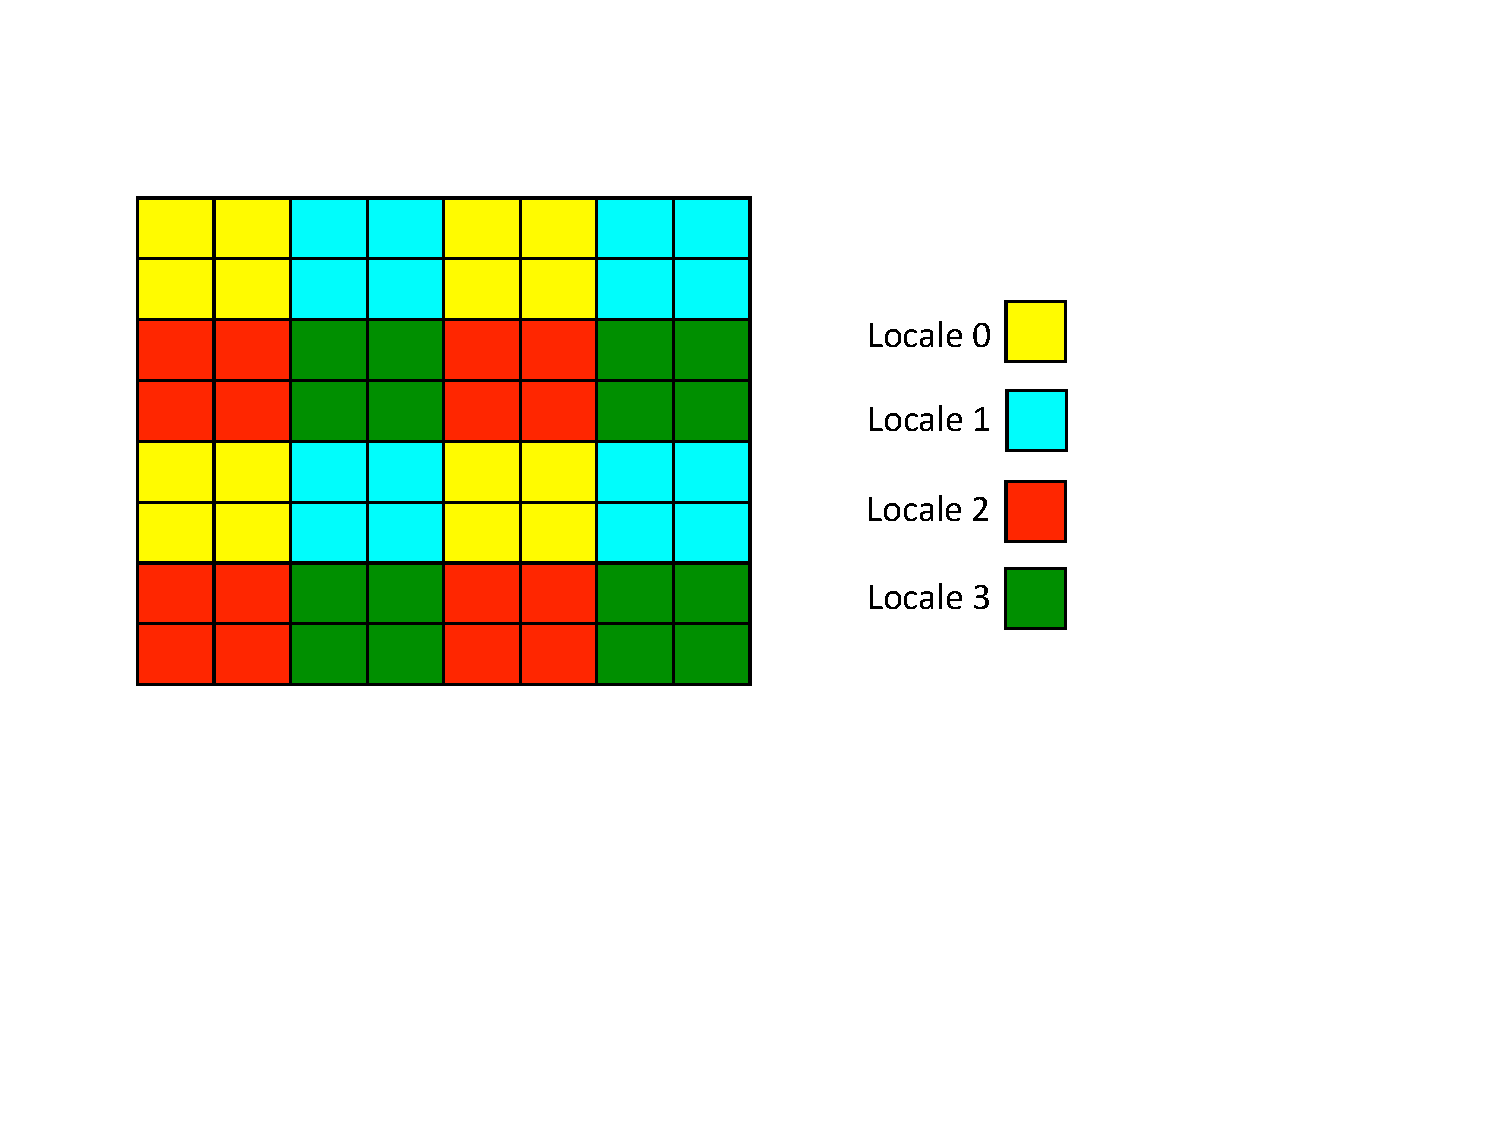
\includegraphics[width=\linewidth]{./Figures/block_cyc_dist}
\caption{Chapel Block Cyclic distribution with a 2 x 2 block size parameter.}
\label{block_cyc_dist}
\end{center}
\end{figure}

The choice of data distribution to use for a program boils down to computation and communication efficiency. Different programs and architectures may require different data distributions. It has been shown that finding an optimal data distribution for parallel processing applications is an NP-complete problem, even for one- or two-dimensional arrays \cite{mace1987memory}. Certain program data access patterns will result in fewer communication calls if the data is distributed in a particular way. For example, many loops in stencil programs that contain nearest neighbor computation will have better communication performance if the data is distributed using a Block distribution. This occurs because on a given loop iteration, the elements accessed are near each other in the array and therefore are more likely to reside on the same locale block. Accessing elements on the same block does not require a remote data access and can be done faster. However, programs that access array elements far away from each other will have better communication performance if data is distributed using a Cyclic distribution. Here, a Block distribution is almost guaranteed to have poor performance because the farther away accessed elements are, the more likely they reside on different locales. 

A programmer may choose a particular data distribution for reasons unknown to the compiler. These reasons may not even take communication behavior into account. For example, Cyclic and Block Cyclic distributions provide better load balancing of data across locales than a Block distribution when array sizes may be changed dynamically because in Cyclic and Block Cyclic distributions, the locales of existing array elements do not change when new array elements are added at the end of the array. In many applications, data redistribution may be needed if elements of a data set are inserted or deleted at the end of the array. In particular, algorithms to redistribute data using a new block size exist for the Block Cyclic distribution \cite{prylli1997fast,walker1996redistribution}. If an application uses a dynamic data set with elements that are appended, a Cyclic or Block Cyclic distribution is superior to Block because new elements are added to the locale that follows the cyclic or block-cyclic pattern. For Block, the entire data set would need to be redistributed every time a new element is appended, which can be expensive. 

\begin{comment}
Compatibility with other PGAS languages might be an important consideration for a programmer when selecting a data distribution. Data sets used by Chapel programs and other PGAS programs should use Cyclic or Block Cyclic distributions because other PGAS languages may not support the Block distribution. A programmer would benefit by distributing the same data set using only one scheme so the data would not have to be replicated for different programs. This is an important consideration for vast data sets that have already been distributed on message passing computers, and we want to perform additional computation on them, perhaps with other programs. 

Therefore in this work, it is our view that the compiler should not change the programmer's choice of data distribution in order to achieve better runtime and communication performance. 
\end{comment}

The compiler should attempt to perform optimizations based on the data distribution that the programmer specified. Our optimization is meant to be applied whenever the programmer specifies a Cyclic or Block Cyclic distribution. It is not applied when the programmer specifies a Block distribution.


\section{Related Work}\label{sec:relwork}

Compilation for distribution memory machines has two main steps: loop optimizations and message passing code generation. First, the compiler performs loop transformations and optimizations to uncover parallelism, improve the granularity of parallelism, and improve cache performance. These transformations include loop peeling, loop reversal, and loop interchange. Chapel is an explicitly parallel language, so uncovering parallelism is not needed. Other loop optimizations to improve the granularity of parallelism and improve cache performance are orthogonal to this paper. The second step is message passing code generation, which includes message aggregation.

Message passing code generation in the traditional model is exceedingly complex, and practical robust implementations are hard to find. These methods \cite{goumas2006message, xue1997communication, callahan1988compiling, ramanujam1991compile} require footprint calculations for each tile. A footprint is the span of data elements accessed by all iterations of a single tile. It is common for a tile's footprint to span across multiple locales, requiring communication between locales. Footprint calculations are modeled by matrices and need to be intersected with the data distribution in order to determine the locality of data elements. Message aggregation can only be done once the compiler determines which data elements of a tile's footprint are remote. These footprint calculations quickly become more complex as the number of locales scales. Our method does not require any footprint calculations, thereby simplifying code generation. 

The polyhedral method is another branch of compiler optimization that seeks to speed up parallel programs on distributed memory architectures \cite{chavarria2005effective, germain1995automatic, Gupta91automaticdata, gupta1996compiling, iancu2008performance, wei1998compiling}. The primary purpose of the polyhedral method is uncovering parallelism and loop optimization, not code generation. Its strength is that it can find sequences of transformations in one step, without searching the entire space of transformations. However, the method at its core does not compute information for message passing code generation. Message passing code generation does not fit the polyhedral model, so ad-hoc methods for code generation have been devised to work on the output of the polyhedral model. However they are no better than corresponding methods in the traditional model, and suffer from many of the same difficulties.

Similar work to take advantage of communication aggregation on distributed arrays has already been done in Chapel. Like distributed parallel loops in Chapel, whole array assignment suffered from locality checks for every array element, even when the locality of certain elements is known in advance. In \cite{sanz2012global}, aggregation was applied to improve the communication performance of whole array assignments for Chapel's Block and Cyclic distributions. Our work goes beyond array assignments and applies aggregation to affine array accesses within parallel loops for Chapel's Cyclic and Block Cyclic distributions. One of the contribution's of \cite{sanz2012global} included two new bulk communication primitives for Chapel developers as library calls, \texttt{chpl\_comm\_gets} and \texttt{chpl\_comm\_puts}. They both rely on the GASNet networking layer, a portion of the Chapel runtime.  Our optimization uses these new communication primitives in our implementation directly to perform bulk remote data transfer between locales.

Extensive work has been done with the UPC compiler (another PGAS language) by \cite{chen2005communication} to improve on its communication performance. This method targets fine-grained communication and uses techniques such as redundancy elimination, split-phase communication, and communication coalescing (similar to message aggregation) to reduce overall communication. However, it is not clear whether this method can be used to improve communication performance across distributed parallel loops. There is no locality analysis that statically determines whether an array access is shared or remote. Our method, modulo unrolling, can determine which accesses are local purely on the affine array access and data distribution. Another major limitation to this work's aggregation scheme is that only contiguous data can be sent in bulk. To aggregate data across an entire loop in a single message, it must be possible to aggregate data elements that are far apart in memory, separated by a fixed stride. Our method handles this by using the strided get and put calls (\texttt{chpl\_comm\_gets} and \texttt{chpl\_comm\_puts}) from \cite{sanz2012global}, described earlier. 

\begin{comment}
\cite{callahan1988compiling}
\cite{chamberlain1998zpl}
\cite{chamberlain1997factor}
\cite{chavarria2005effective}
\cite{davidson1995improving}
\cite{Dion96compilingaffine}
\cite{germain1995automatic}
\cite{Gupta91automaticdata}
\cite{gupta1996compiling}
\cite{huang1994speculative}
\cite{iancu2008performance}
\cite{li1991data}
\cite{pouchet2011loop}
\cite{ramanujam1991compile}
\cite{shih2000efficient}
\cite{trifunovic2010graphite}
\cite{wei1998compiling}
\cite{chamberlain2011user}
\cite{bonachea2007proposal}
\cite{sanz2012global}
\end{comment}
\section{Background on Modulo Unrolling}\label{sec:modulo_unrolling}

Modulo unrolling \cite{barua1999maps} is a static disambiguation method used in tiled architectures that is applicable to loops with affine array accesses. An affine function of a set of variables is defined as a linear combination of those variables. An affine array access is any array access where each dimension of the array is accessed by an affine function of the loop induction variables. For example, for loop index variables $i$ and $j$ and array $A$, $A[i+2j+3][2j]$ is an affine access, but $A[ij+4][j^2]$ and $A[2i^2+1][ij]$ are not. 

Modulo unrolling works by unrolling the loop by a factor equal to the number of memory banks on the architecture. If the arrays accessed within the loop are distributed using low-order interleaving (a Cyclic distribution), then after unrolling, each array access will be \textit{statically disambiguated}, or guaranteed to reside on a single bank for all iterations of the loop. This is achieved with a modest increase of the code size. 

\begin{figure}
\begin{center}
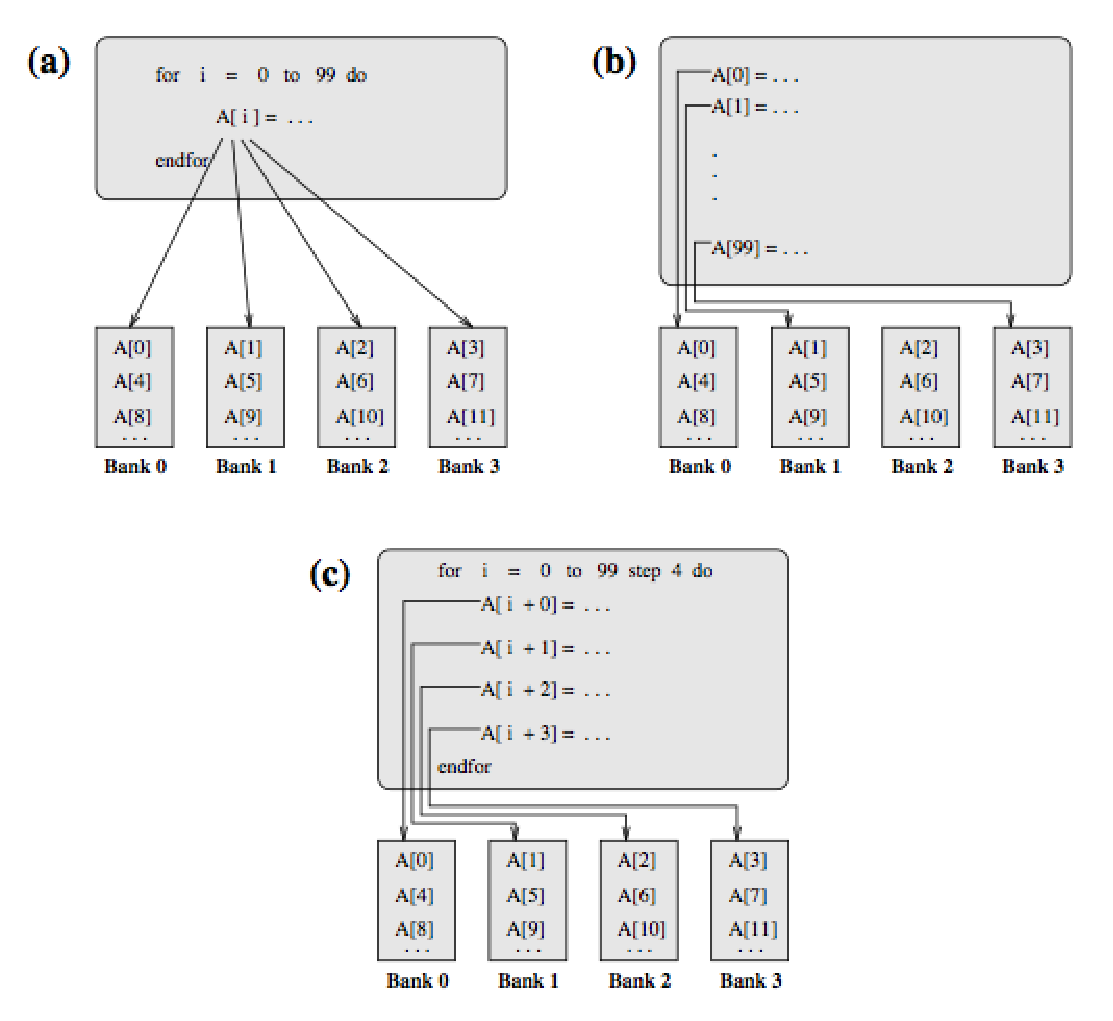
\includegraphics[width=\linewidth]{./Figures/modulo_unrolling.eps}
\caption{Modulo unrolling example. (a) Original sequential for loop. Array $A$ is distributed using a Cyclic distribution. Each array access maps to a different memory bank on successive loop iterations. (b) Fully unrolled loop. Trivially, each array access maps to a single memory bank because each access only occurs once. This loop dramatically increases the code size for loops traversing through large data sets. (c) Loop transformed using modulo unrolling. The loop is unrolled by a factor equal to the number of memory banks on the architecture. Now each array access is guaranteed to map to a single memory bank for all loop iterations and code size increases only by the loop unroll factor.}
\label{modulo_unrolling}
\end{center}
\end{figure}

To understand modulo unrolling, refer to Figure~\ref{modulo_unrolling}. In Figure~\ref{modulo_unrolling}a there is a code fragment consisting of a sequential \textbf{for} loop with a single array access $A[i]$. The array $A$ is distributed over four memory banks using a Cyclic distribution. As is, the array $A$ is not statically disambiguated because accesses of $A[i]$ go to different memory banks on different iterations of the loop. The array access $A[i]$ has bank access patterns 0, 1, 2, 3, 0, 1, 2, 3, ... in successive loop iterations. 

A naive approach to achieving static disambiguation is to fully unroll the loop, as shown in Figure~\ref{modulo_unrolling}b. Here, the original loop is unrolled by a factor of 100. Because each array access is independent of the loop induction variable $i$, static disambiguation is achieved trivially. Each array access resides on a single memory bank. However, fully unrolling the loop is not an ideal solution to achieving static disambiguation because of the large increase in code size. This increase in code size is bounded by the unroll factor, which may be extremely large for loops iterating over large arrays. Fully unrolling the loop may not even be possible for a loop bound that is unknown at compile time. 

A more practical approach to achieving static disambiguation without a dramatic increase in code size is to unroll the loop by a factor equal to the number of banks on the architecture. This is shown in Figure~\ref{modulo_unrolling}c and is known as \textit{modulo unrolling}. Since we have 4 memory banks in this example, we unroll the loop by a factor of 4. Now every array reference in the loop maps to a single memory bank on all iterations of the loop. Specifically, $A[i]$ refers to bank 0, $A[i+1]$ refers to bank 1, $A[i+2]$ refers to bank 2, and $A[i+3]$ refers to bank 3. The work in \cite{barua1999maps} shows that an unroll factor providing this property always exists not only for the code in Figure \ref{modulo_unrolling}, but for the general case of any affine function in a loop.  The unroll factor may not always equal the number of banks, but a suitable unroll factor can always be computed.

Modulo unrolling, as used in \cite{barua1999maps} provides static disambiguation and memory parallelism for tiled architectures. That is, after unrolling, each array access can be done in parallel because array accesses map to a different memory banks. 
\section{Motivation for Message Aggregation}\label{sec:motivation_for_aggregation} 

In Chapel, a program's data access patterns and the programmer's choice of data distribution greatly influence the program's runtime and communication behavior. There are some situations where programs exhibit predictable patterns of communication that the compiler can detect. In doing so, the compiler can aggregate remote data elements coming from one locale into one local buffer via a single message and then access this local buffer on subsequent iterations of the loop. 

For example, consider Chapel code for the Jacobi computation shown in Figure \ref{jacobi_code}, a common stencil operation that computes elements of a two dimensional array as an average of that element's four adjacent neighbors. On each iteration of the loop, five array elements are accessed in an affine manner: the current array element $A_{new}[i, j]$ and its four adjacent neighbors $A[i+1, j]$, $A[i-1, j]$, $A[i, j+1]$, and $A[i, j-1]$. Naturally, the computation will take place on the locale of $A_{new}[i, j]$, the element being written to. If arrays $A$ and $A_{new}$ are distributed with a Cyclic distribution as shown in Figure \ref{cyc_dist}, then it is guaranteed that $A[i+1, j]$, $A[i-1, j]$, $A[i, j+1]$, and $A[i, j-1]$ will not reside on the same locale as $A_{new}[i, j]$ \textbf{for all iterations of the loop}. These remote elements are transferred over to $A_{new}[i, j]$'s locale in four individual messages during every loop iteration. For large data sets, transferring four elements individually per loop iteration drastically slows down the program because the message overhead is incurred more than once. 

Since the data is distributed using a Cyclic distribution, we notice that the data is accessed in the same way every cycle. For example, on iteration $(2, 2)$, $A_{new}[2, 2]$ resides on locale 3, $A[2, 1]$ and $A[2, 3]$ reside on locale 1, and $A[1, 2]$ and $A[3, 2]$ reside on locale 2. If we look at iteration $(4, 2)$ which is an iteration in the next cycle, we see that $A_{new}[4, 2]$ also resides on locale 3, $A[4, 1]$ and $A[4, 3]$ reside on locale 1, and $A[3, 2]$ and $A[5, 2]$ reside on locale 2. We can therefore bring in all remote data elements accessed by iterations where $A_{new}[i, j]$ resides on locale 3 to locale 3 before the loop executes and write them back to locales 1 and 2 after the loop finishes. 

If we focus on locale 3, there will be four buffers containing remote data elements after aggregation has occurred, one for each affine array access in the loop in Figure \ref{jacobi_code}. The first buffer is known conceptually as $buf$\_$north$ and will contain the array slice $A[2..7$ $by$ $2, 1..6$ $by$ $2]$. The elements in this buffer correspond to all elements produced by the $A[i, j-1]$ array access over all iterations of the loop in Figure \ref{jacobi_code} where $A_{new}[i, j]$ also resides on locale 3. Similarly, there are buffers $buf$\_$south$, $buf$\_$east$, and $buf$\_$west$ that contain a similar description of elements for array accesses $A[i, j+1]$, $A[i+1, j]$, and $A[i-1, j]$ respectively. Now that a copy of all remote data elements reside on the locale that they are used from, the affine array accesses other than $A_{new}[i, j]$ can be replaced with accesses to the local buffers. After the loop has finished, any buffer elements that have been written to are communicated back to their respective remote locales in their own aggregate messages. This optimization can also be applied to the Block Cyclic distribution, as the data access pattern is the same for elements in the same position within a block. 

If arrays $A$ and $A_{new}$ are instead distributed using Chapel's Block or Block Cyclic distributions as shown in Figure \ref{block_dist} and Figure \ref{block_cyc_dist} respectively, the program will only perform remote data accesses on iterations of the loop where element $A_{new}[i, j]$ is on the boundary of a block. As the blocksize increases, the number of remote data accesses for the Jacobi computation decreases. For the Jacobi computation, it is clear that distributing the data using Chapel's Block distribution is the best choice in terms of communication. Executing the program using a Block distribution will result in fewer remote data accesses than when using a Block Cyclic distribution. Similarly, executing the program using a Block Cyclic distribution will result in fewer remote data accesses than when using a Cyclic distribution. 

It is important to note that the Block distribution is not the best choice for all programs using affine array accesses. Programs with strided access patterns that use a Block distribution will have poor communication performance because accessed array elements are more likely to reside outside of a block boundary. For these types of programs, a Cyclic or Block Cyclic distribution will perform better. 

\section{Message Aggregation Loop Optimization for Parallel Affine Loops}\label{sec:transformation} 

This section describes our method to transform an affine loop that computes on cyclically or block-cyclically distributed data into an equivalent loop that performs message aggregation. As described in Section \ref{sec:data_distributions}, our method is not meant for block distributed data. The proposed method is based on modulo unrolling \cite{barua1999maps}, described in Section \ref{sec:modulo_unrolling}. Here we describe the method in pseudocode for simplicity and to show that this method is applicable to languages other than Chapel. 

\begin{figure}
\begin{center}
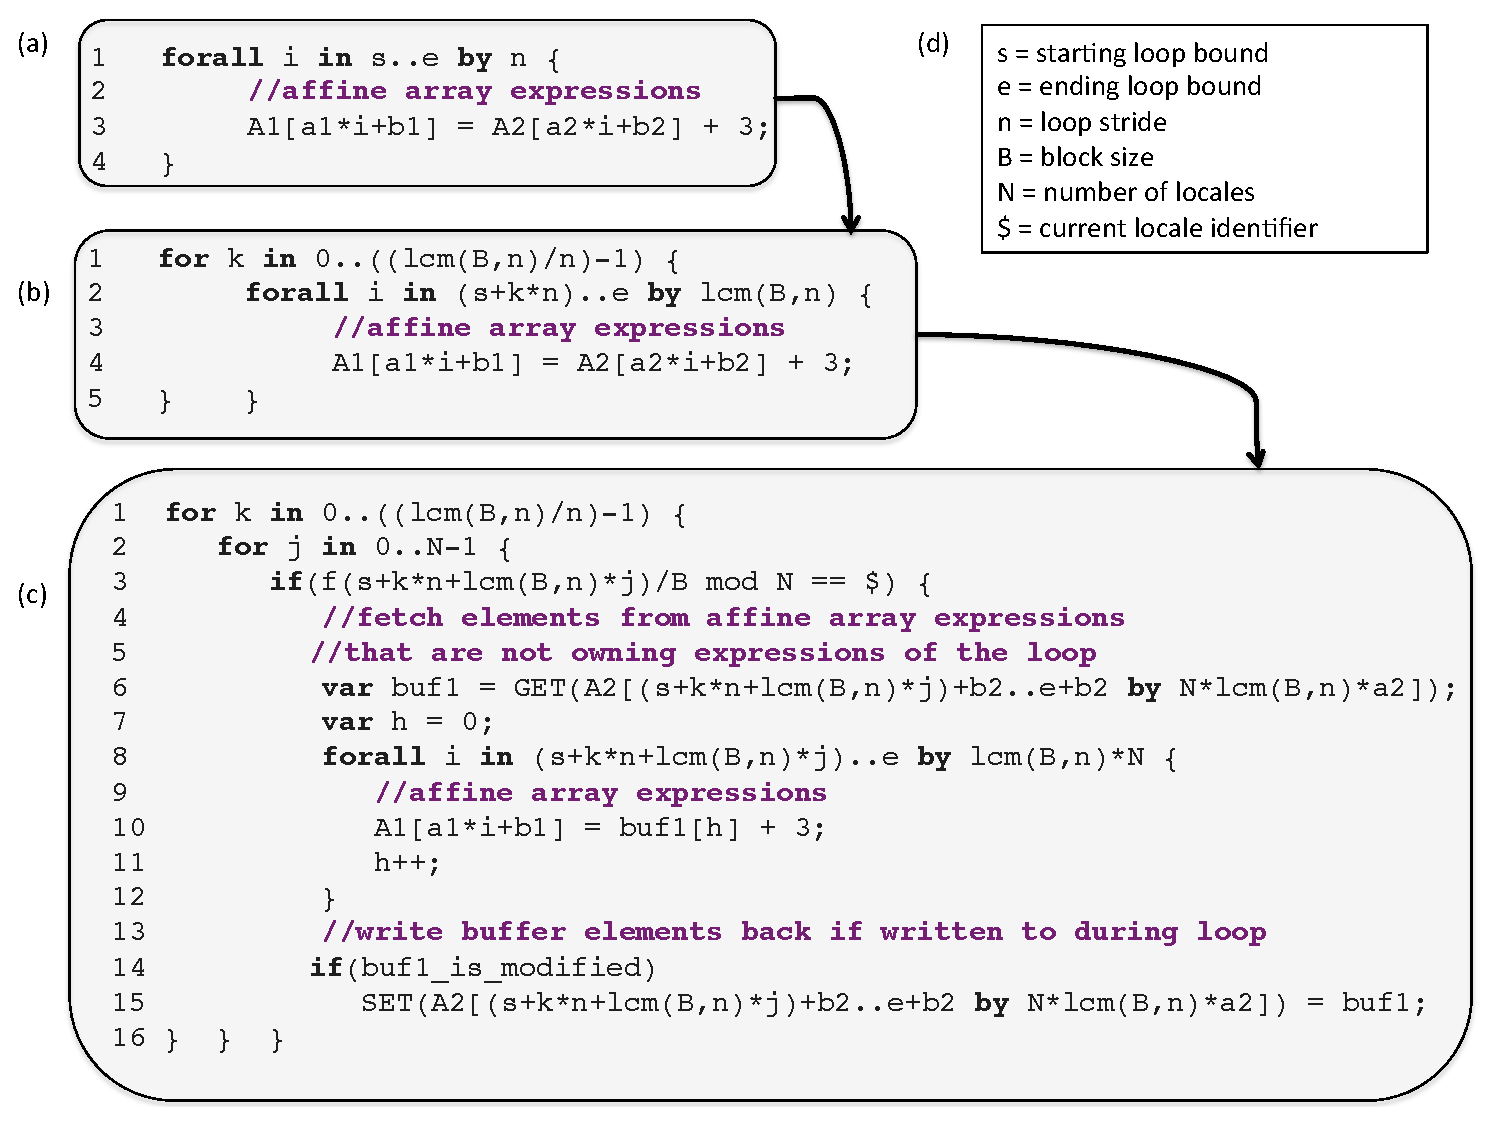
\includegraphics[scale=0.35]{./Figures/transformations}
\caption{Steps to transform a parallel affine loop where the data is distributed cyclically or block-cyclically into an equivalent loop that performs message aggregation. (a) Original distributed parallel loop with two affine array accesses. (b) Loop after Block Cyclic transformation. After this step, the affine array accesses in loops with data distributed block-cyclically will be statically disambiguated. (c) Loop after the owning expression calculation and message aggregation steps. In line 6, remote array elements are communicated to a local buffer before the loop. The affine array access for $A_{2}$ is replaced with an access to the local buffer in line 10. In lines 14-15, elements in the local buffer are written back to the remote locale if they are written to during the loop. (d) Key of symbolic variables used in the transformations in parts a-c. }
\label{transformations}
\end{center}
\end{figure}

\subsection{Modulo Unrolling Without Unrolling}\label{subsec:modulo_unrolling_without_unrolling}

Modulo unrolling increases code size because it unrolls loops by a factor equal to the number of locales (memory banks) on the system. However, we have devised an adaptation called modulo unrolling WU for message passing machines that does not increase code size. To understand it, consider that for parallel machines that use message passing, static disambiguation can be achieved by using the locale identifier without increasing the code size. Conceptually, an affine loop written in source code on a message passing machine where data is distributed cyclically among four locales such as:\newline

\tab{\texttt{\textbf{forall} i \textbf{in} 0..99 \{}}

\tab{\tab{\texttt{A[i] = B[i+2];}}}

\tab{\texttt{\}}}\newline

becomes statically disambiguated using this observation as follows:\newline

\tab{\texttt{\textbf{forall} i \textbf{in} 0..99 \textbf{by} 4 \{}}

\tab{\tab{\texttt{A[i+\$] = B[i+2+\$];}}}

\tab{\texttt{\}}}\newline

where \$ represents the locale identifier. The above is the code that is run on each locale. This transformation is called \textit{modulo unrolling without unrolling (modulo unrolling WU)} since, like modulo unrolling, it can be used for static disambiguation but on message passing machines instead of tiled architectures. Here, no unrolling of the loop is necessary.

Figure \ref{transformations} shows how a generalized affine loop, expressed symbolically, can be transformed by our method in three steps: the Block Cyclic transformation (Figure \ref{transformations}a $\rightarrow$ Figure \ref{transformations}b), the owning expression calculation (described in Section \ref{subsec:owning_expression_calculation}), and the message aggregation (Figure \ref{transformations}b $\rightarrow$ Figure \ref{transformations}c). 

As shown in Figure \ref{transformations}a, our method takes as its input a parallel \textbf{forall} loop that contains a number of affine array expressions in its loop body. Non-affine expressions are allowed in the loop body, but they are not optimized. The input loop shown in Figure \ref{transformations}a is defined by three explicit parameters: the starting loop bound $s$, the ending loop bound $e$, and the loop stride $n$. The input loop also contains two implicit parameters based on the data distribution. The number of locales the data is distributed over is $N$, and the block size, the number of consecutive array elements allocated to a single locale, is $B$. All five parameters are elements of $\mathbb{N}$. The output of the optimization is an equivalent loop structure that aggregates communication from all of the loop body's remote affine array accesses.

\subsection{Block Cyclic Transformation}\label{subsec:block_cyclic_transformation}

Modulo unrolling as described in \cite{barua1999maps} guarantees static disambiguation for data distributed cyclically but not for block-cyclically distributed data. However, we can think of a Block Cyclic distribution as $B$ adjacent Cyclic distributions, each with a cycle size that is greater than $N$. In order to achieve static disambiguation for the Block Cyclic distribution, we must transform input loops with $B >$ 1 into an equivalent loop with a loop step size that is a multiple of $B$. 

Lines 1 and 2 of Figure \ref{transformations}b show this transformation. We replace the loop step size on line 1 of Figure \ref{transformations}a with the \textit{least common multiple} of $B$ and $n$ in line 2 of Figure \ref{transformations}b. The intuition behind this new step size is that two successive loop iterations accessing the same position within a block will always be separated by a fixed stride length that is a multiple of the block size. To maintain the original meaning of the input loop, an outer \textbf{for} loop is added on line 1 of Figure \ref{transformations}b to handle iterations within each block, and the starting loop bound on line 2 is written in terms of the outer loop variable $k$. After this transformation, all affine array accesses in the loop with be statically disambiguated. This transformation is a variant of the well-known strip mining transformation, which has been used for many other purposes in the literature.

The Cyclic and Block Cyclic distributions are closely related. Any Cyclic distribution can be thought of as a Block Cyclic distribution with $B$ = 1. If we apply the transformation in Figure \ref{transformations}b to a loop with cyclically distributed data, we will end up with the original input loop in Figure \ref{transformations}a, which is already statically disambiguated after applying the transformation described in Section \ref{subsec:modulo_unrolling_without_unrolling}. 

\subsection{Owning Expression Calculation}\label{subsec:owning_expression_calculation}

There may be many affine array accesses in the input loop, each mapped to a single locale after static disambiguation. For the best communication performance, we must determine the \textit{owning expression} for the loop, which is the most common affine array expression in the loop body. More formally, the owning expression is an affine function $f(i)$, where $i$ is the loop's induction variable, that occurs statically the most number of times in the loop body. We can then use the owning expression to assign loop iterations to locales. Note that there may be instances where affine array expressions are found within control flow statements inside the loop body. Here, we will not know how many times each condiitonal block will execute at compile time. For these cases, we can use static profiling methods described in \cite{wu1994static} to estimate the occurrences of affine array accesses within conditional blocks in the loop body.  

As an example of how the owning expression is computed and used, consider that there are two affine array accesses in Figure \ref{transformations}b: $A_{1}[a_{1}i+b_{1}]$ and $A_{2}[a_{2}i+b_{2}]$. Each appears once in the loop body, so either expression can be chosen as the owning expression for the loop. For the remainder of Figure \ref{transformations}, we assume that $a_{1}i+b_{1}$ is the owning expression. 

Line 3 of Figure \ref{transformations}c shows symbolically how the owning expression, which is an affine function of the loop induction variable $i$, is used to ensure that loop iterations are assigned to locales such that most of the affine array accesses are local. The argument to the owning expression $f$ in line 3 represents the first loop iteration in each strip-mined portion created in the Block Cyclic transformation. We evaluate the owning expression at this loop iteration. This yields the array index that is most accessed during this loop iteration. The locale where this array index resides should be responsible for handling all iterations in this strip-mined portion because this way most of the loop body's affine array accesses will be local.

\subsection{Message Aggregation}\label{subsec:message_aggregation}

\begin{comment}
This whole writing is very confusing since it is observational, where it simply observes some points about the code. Please write this text to be deductive, meaning you should start with a goal, and then saying how this code meets that goal. (This would also make the text more top down.)

In this case, the goal is to communicate the non-owned accesses, which in this case is the A2[a2*i + b2] access. State that as the goal at the beginning, and then say which portions are remote, and how we generate code to get those portions.
\end{comment}

The final step of the optimization is to communicate the non-owned remote affine array accesses in a single message before the loop. Figure \ref{transformations}c shows this transformation. The loop nest starting on line 2 symbolically represents which loop iterations are assigned to the $N$ locales on the system based on the owning expression calculation (line 3). The array access $A_{2}[a_{2}i+b_{2}]$ is non-owned and may either be entirely remote or entirely local. If entirely remote (as is assumed here), it will require communication. We compute its corresponding remote array slice in line 6 before communicating the entire array slice to a local buffer. Modulo unrolling guarantees that all elements in this array slice are remote with respect to a single locale on the loop iterations that they are used. So, they can be brought to the current locale \$ in one message. Now in lines 8-12, the affine array access $A_{2}[a_{2}i+b_{2}]$ can be replaced with an access to the local buffer. Lines 14-15 handle the case that elements brought over in bulk need to be written back to their remote locale. 

\subsection{Loops with Multi-Dimensional Array Accesses}\label{subsec:multi_dimensional}

The series of transformations described in this section and illustrated in Figure \ref{transformations} all apply to one-dimensional arrays indexed by one loop induction variable. These transformations can also be generalized to apply to certain affine array accesses for multi-dimensional arrays. The intuition for this generalization is as follows. The input affine loop now contains $m$ loop induction variables $i_{1}$, $i_{2}$, ... , $i_{m}$. Similarly, there are now $m$ starting loop bounds, ending loop bounds, loop strides, and block sizes. The $p^{th}$ block size is now the number of consecutive array elements allocated to a single locale in dimension $p$ of the array, where $1 \le p \le m$. Each affine array access in the loop body now contains $m$ affine array expressions where expression $p$ is an affine function of $i_{p}$. 

Under these assumptions, the transformations described in this section need only be applied to each loop induction variable independently. The owning expression calculation now produces an $m$-tuple of affine array expressions.\footnote{In our adaptation of modulo unrolling WU in Chapel, the Cyclic distribution can apply the optimization to loops with multi-dimensional array accesses, but the Block Cyclic distribution is limited to one-dimensional array accesses because of the current limitations within Chapel's existing Block Cyclic implementation that are outside the scope of this work. } The results we collect in this work consider one-, two-, and three-dimensional array accesses. 





%\section{Chapel Language Features Necessary for Modulo Unrolling}\label{sec:language_features}

The goal of this section is to provide a basic understanding of zippered iteration and array slicing in Chapel and to show how the modulo unrolling optimization described in Sections \ref{sec:motivation_for_aggregation}, \ref{sec:cyclic_modulo}, and \ref{sec:block_cyclic_modulo} fits in naturally with these language constructs. Any parallel loop with affine array accesses can be written using zippered iteratiors and array slicing. Therefore, parallel iteratiors are candidates within the language to implement the optimization.

\subsection{Zippered Iteration}\label{sec:zippered_iteration}

Iterators are a widely used language feature in the Chapel programming language. Chapel iterators are blocks of code that are similar to functions and methods except that iterators can return multiple values back to the call site with the use of the \textit{yield} keyword instead of \textit{return}. Iterators are commonly used in loops to traverse data structures in a particular fashion. For example, an iterator $fibonacci(n: int)$ might be responsible for yielding the first $n$ Fibonacci numbers. This iterator could then be called in a loop's header to execute iterations 0, 1, 1, 2, 3, and so on. Arrays themselves are iterable in Chapel by default. 

Chapel allows multiple iterators of the same size and shape to be iterated through simultaneously. This is known as \textit{zippered iteration} \cite{chamberlain2011user}. When zippered iteration is used, corresponding iterations are processed together. On each loop iteration, an $n$-tuple is generated, where $n$ is the number of items in the zippering. The $d^{th}$ component of the tuple generated on loop iteration $j$ is the $j^{th}$ item that would be yielded by iterator $d$ in the zippering. 

Zippered iteration can be used with either sequential \textbf{for} loops or parallel \textbf{forall} loops in Chapel. Parallel zippered iteration is implemented in Chapel using leader-follower semantics. That is, a \textit{leader} iterator is responsible for creating tasks and dividing up the work to carry out the parallelism. A \textit{follower} iterator performs the work specified by the leader iterator for each task and generally resembles a serial iterator. 

\subsection{Array Slicing}\label{sec:array_slicing}

Chapel supports another useful language feature known as \textit{array slicing}. This feature allows portions of an array to be accessed and modified in a succinct fashion. For example, consider two arrays $A$ and $B$ containing indices from $1..10$. Suppose we wanted to assign elements $A[6]$, $A[7]$, and $A[8]$ to elements $B[1]$, $B[2]$, and $B[3]$ respectively. We could achieve this in one statement by writing $B[1..3] = A[6..8]$. Here, $A[6..8]$ is a slice of the original array $A$, and $B[1..3]$ is a slice of the original array $B$. In Chapel, an array slice can support a range of elements with a stride in some cases. For example, in the previous example, we could have made the assignment $B[1..3] = A[1..6$ $by$ $2]$. This would have assigned elements $A[1]$, $A[3]$, and $A[5]$ to elements $B[1]$, $B[2]$, and $B[3]$ respectively. Since all array slices in Chapel are arrays themselves, array slices are also iterable. 

Together, array slicing and parallel zippered iteration can express any parallel affine loop in Chapel that uses affine array accesses. Each affine array access in the loop body is replaced with a corresponding array slice in the loop header, which produces the same elements as the original loop. Consider the code fragment in Figure \ref{affine_loop}a. There are two affine array accesses $A[i]$ and $B[i+2]$ in Figure \ref{affine_loop}a. The loop is written in a standard way where the loop induction variable $i$ takes on values from 1 to 10. Because the loop is a \textbf{forall} loop, loop iterations are not guaranteed to complete in a specific order. This loop assigns elements of array $B$ to $A$ such that the $i^{th}$ element of $A$ is equal to the $(i+2)^{th}$ element of $B$ after the loop finishes. In Figure \ref{affine_loop}b, the same loop is written using zippered iterators. The loop induction variable $i$ no longer needs to be specified, and each affine array access has been replaced with an array slice in the zippering of the loop header. It is possible to transform an affine loop in this fashion even when an affine array access has a constant factor multiplied by the loop induction variable. The resulting array slice will contain a stride equal to the constant factor. The two loops in FIgure \ref{affine_loop} are equivalent and generate the same results, but they differ in their execution.

Because any parallel affine loop can be transformed into an equivalent parallel loop that uses zippered iteration, we observe a natural place in the Chapel programming language in which to implement modulo unrolling: the leader and follower iterators of the Cyclic and Block Cyclic distribution. The leader iterator divides up the loop's iterations according to the locales they are executed on and passes this work to each follower iterator in the zippering. The follower iterator can then perform the aggregation of remote data elements according to the work that has been passed to it. 

\begin{comment}
\begin{figure}
	\begin{center}
	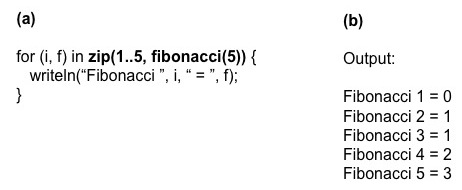
\includegraphics[scale=0.60]{./Figures/zippered_iteration}
	\caption{(a) Chapel code fragment showing a loop using zippered iteration. A tuple of loop index variables equal to the number of items in the zippering is declared in the loop header. If $j$ is the current loop iteration, variable $i$ is equal to the $j^{th}$ element in the range $1..5$, and $f$ corresponds to the $j^{th}$ element in the iterator $fibonacci(5)$. The \textit{zip} keyword tells the loop header which items to iterate over using zippered iteration. (b) Program output of the code fragment in Figure~\ref{zippered_iteration}a.}
	\label{zippered_iteration}
	\end{center}
\end{figure}
\end{comment}

\begin{figure}
	\begin{center}
	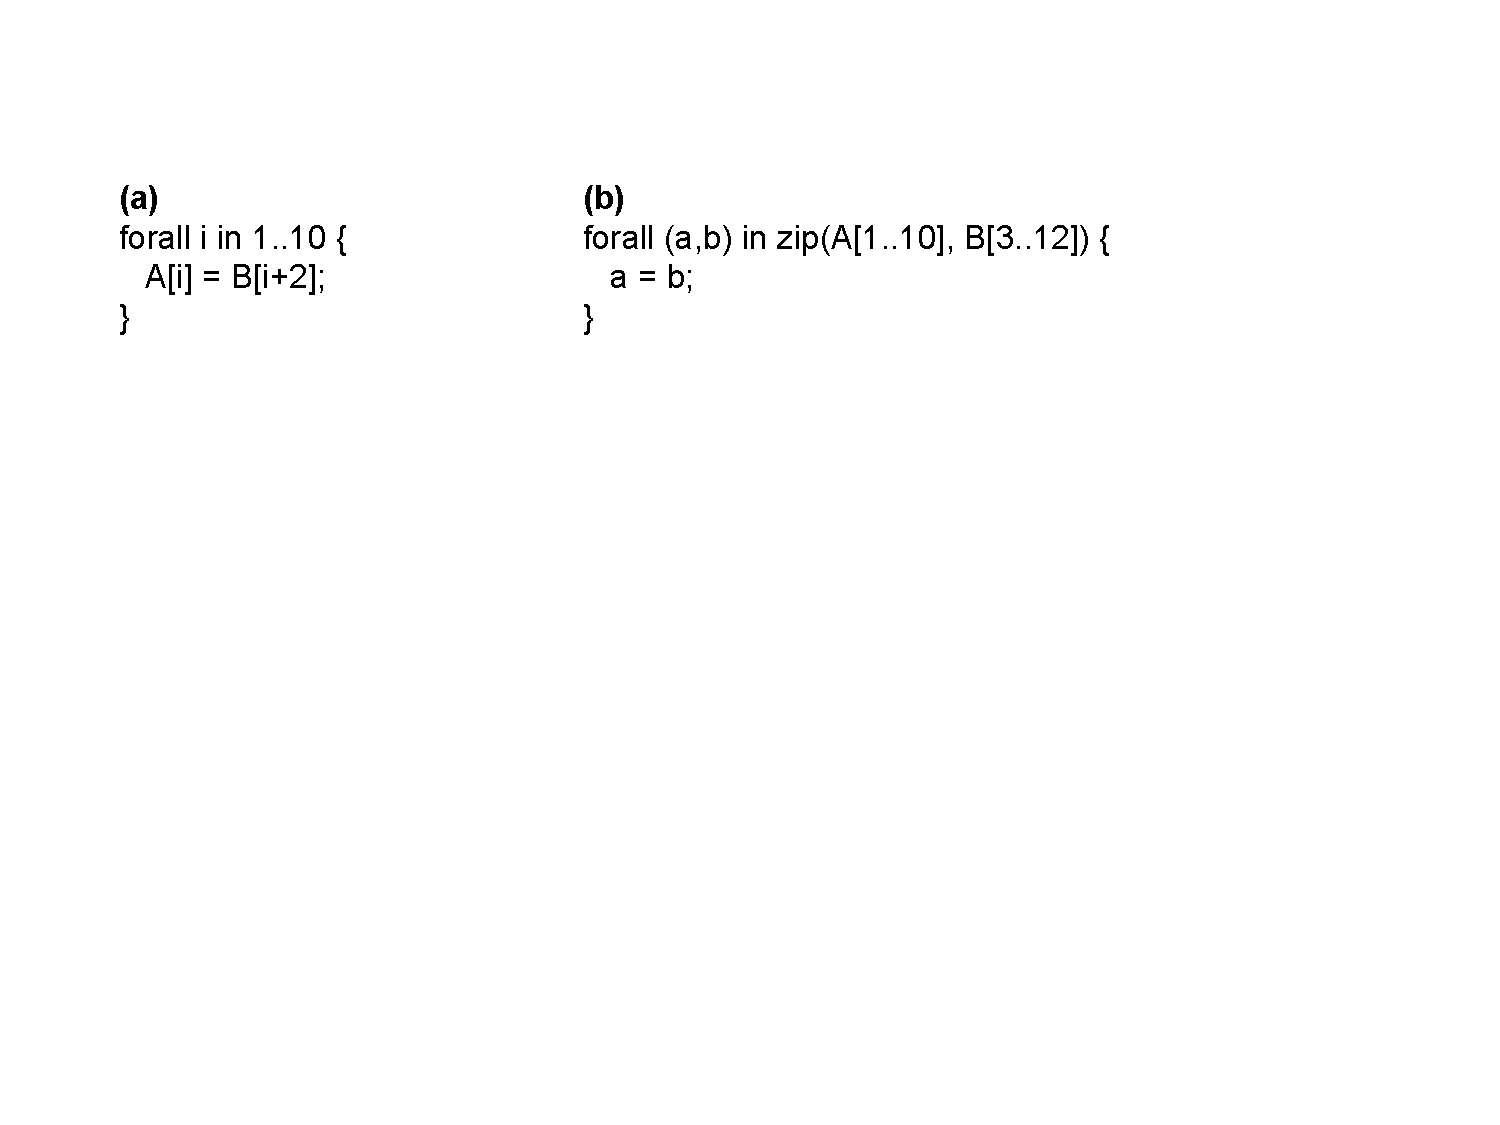
\includegraphics[scale=0.50]{./Figures/affine_loop}
	\caption{(a) Chapel loop written using a single loop induction variable $i$ ranging from 1 to 10. The loop contains two affine array accesses. (b) The same loop written using zippered iterators in Chapel. Instead of a loop induction variable and a range of values to denote the loop bounds, two array slices each containing the 10 elements accessed by the loop in (a) are specified.}
	\label{affine_loop}
	\end{center}
\end{figure}


\section{Adaptation in Chapel}\label{sec:adaptation_in_chapel}

%\section{Chapel Language Features Necessary for Modulo Unrolling}\label{sec:language_features}

The goal of this section is to present our adaptation in Chapel of the modulo unrolling WU optimization presented in Section \ref{sec:transformation}. We also provide a basic understanding of zippered iteration and array slicing, two important features in Chapel used in the optimization's implementation. 

\subsection{Chapel Zippered Iteration}\label{sec:zippered_iteration}

Iterators are a widely used language feature in the Chapel programming language. Chapel iterators are blocks of code that are similar to functions and methods except that iterators can return multiple values back to the call site with the use of the \textit{yield} keyword instead of \textit{return}. Iterators are commonly used in loops to traverse data structures in a particular fashion. For example, an iterator $fibonacci(n: int)$ might be responsible for yielding the first $n$ Fibonacci numbers. This iterator could then be called in a loop's header to execute iterations 0, 1, 1, 2, 3, and so on. Arrays themselves are iterable in Chapel by default. This is how Chapel can support other important language features such as scalar promotion and whole array assignment. 

Chapel allows multiple iterators of the same size and shape to be iterated through simultaneously. This is known as \textit{zippered iteration} \cite{chamberlain2011user}, and an example is shown in Figure \ref{affine_loop}b. When zippered iteration is used, corresponding iterations are processed together. On each loop iteration, an $n$-tuple is generated, where $n$ is the number of items in the zippering. The $d^{th}$ component of the tuple generated on loop iteration $j$ is the $j^{th}$ item that would be yielded by iterator $d$ in the zippering. 

Zippered iteration can be used with either sequential \textbf{for} loops or parallel \textbf{forall} loops in Chapel. Parallel zippered iteration is implemented in Chapel using leader-follower semantics. That is, a \textit{leader} iterator is responsible for creating tasks and dividing up the work to carry out the parallelism. A \textit{follower} iterator performs the work specified by the leader iterator for each task and generally resembles a serial iterator. 

\subsection{Chapel Array Slicing}\label{sec:array_slicing}

Chapel supports another useful language feature known as \textit{array slicing}. This feature allows portions of an array to be accessed and modified in a succinct fashion. For example, consider two arrays $A$ and $B$ containing indices from $1..10$. Suppose we wanted to assign elements $A[6]$, $A[7]$, and $A[8]$ to elements $B[1]$, $B[2]$, and $B[3]$ respectively. We could achieve this in one statement by writing $B[1..3] = A[6..8]$. Here, $A[6..8]$ is a slice of the original array $A$, and $B[1..3]$ is a slice of the original array $B$. 

In Chapel, an array slice can support a range of elements with a stride in some cases. For example, in the previous example, we could have made the assignment $B[1..3] = A[1..6$ $by$ $2]$. This would have assigned elements $A[1]$, $A[3]$, and $A[5]$ to elements $B[1]$, $B[2]$, and $B[3]$ respectively. Since all array slices in Chapel are arrays themselves, array slices are also iterable. 

\begin{figure}
	\begin{center}
	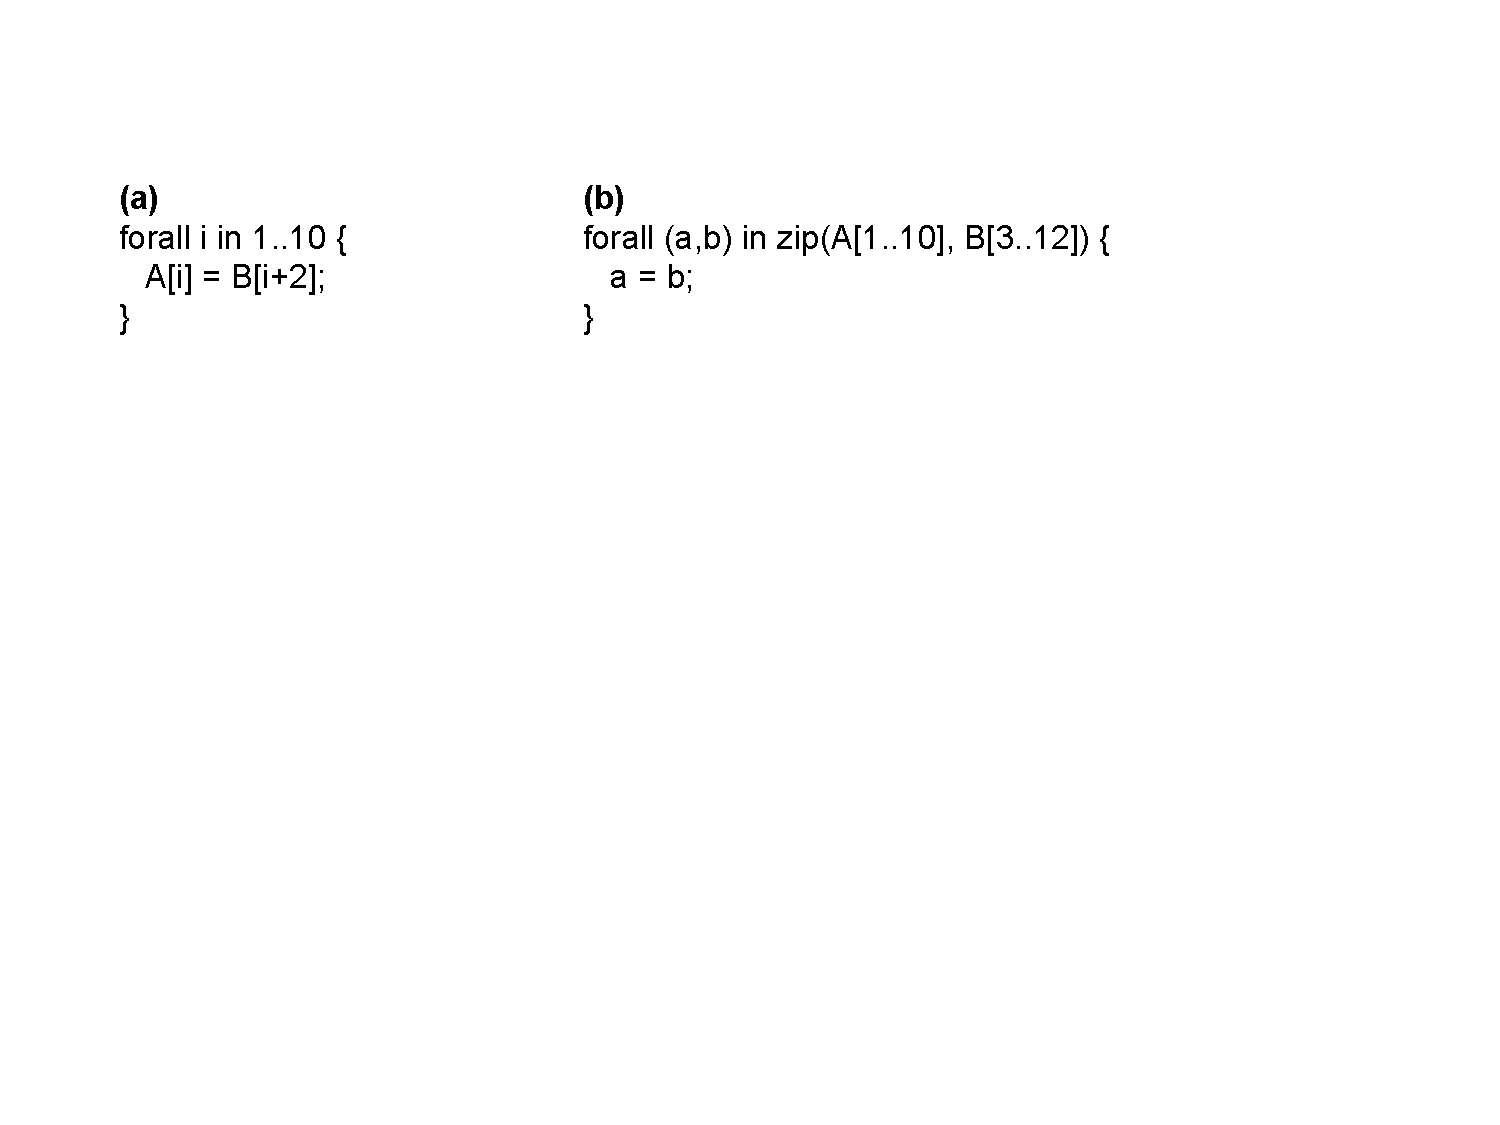
\includegraphics[scale=0.50]{./Figures/affine_loop}
	\caption{(a) Chapel loop written using a single loop induction variable $i$ ranging from 1 to 10. The loop contains two affine array accesses. (b) The same loop written using zippered iterators in Chapel. Instead of a loop induction variable and a range of values to denote the loop bounds, two array slices each containing the 10 elements accessed by the loop in (a) are specified.}
	\label{affine_loop}
	\end{center}
\end{figure}

Together, array slicing and parallel zippered iteration can express any parallel affine loop in Chapel that uses affine array accesses. Each affine array access in the loop body is replaced with a corresponding array slice in the loop header, which produces the same elements as the original loop. 

Consider the code fragment in Figure \ref{affine_loop}a. There are two affine array accesses $A[i]$ and $B[i+2]$ in Figure \ref{affine_loop}a. The loop is written in a standard way where the loop induction variable $i$ takes on values from 1 to 10. Because the loop is a \textbf{forall} loop, loop iterations are not guaranteed to complete in a specific order. This loop assigns elements of array $B$ to $A$ such that the $i^{th}$ element of $A$ is equal to the $(i+2)^{th}$ element of $B$ after the loop finishes. In Figure \ref{affine_loop}b, the same loop is written using zippered iterators. The loop induction variable $i$ no longer needs to be specified, and each affine array access has been replaced with an array slice in the zippering of the loop header. It is possible to transform an affine loop in this fashion even when an affine array access has a constant factor multiplied by the loop induction variable. The resulting array slice will contain a stride equal to the constant factor. The two loops in Figure \ref{affine_loop} are equivalent and generate the same results, but they differ in their execution.

Because any parallel affine loop can be transformed into an equivalent parallel loop that uses zippered iteration, we observe a natural place in the Chapel programming language in which to implement modulo unrolling WU: the leader and follower iterators of the Cyclic and Block Cyclic distribution. The leader iterator divides up the loop's iterations according to the locales they are executed on and passes this work to each follower iterator in the zippering. The follower iterator can then perform the aggregation of remote data elements according to the work that has been passed to it. 

\begin{comment}
\begin{figure}
	\begin{center}
	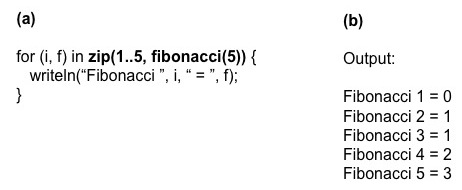
\includegraphics[scale=0.60]{./Figures/zippered_iteration}
	\caption{(a) Chapel code fragment showing a loop using zippered iteration. A tuple of loop index variables equal to the number of items in the zippering is declared in the loop header. If $j$ is the current loop iteration, variable $i$ is equal to the $j^{th}$ element in the range $1..5$, and $f$ corresponds to the $j^{th}$ element in the iterator $fibonacci(5)$. The \textit{zip} keyword tells the loop header which items to iterate over using zippered iteration. (b) Program output of the code fragment in Figure~\ref{zippered_iteration}a.}
	\label{zippered_iteration}
	\end{center}
\end{figure}
\end{comment}

\begin{figure}
	\begin{center}
	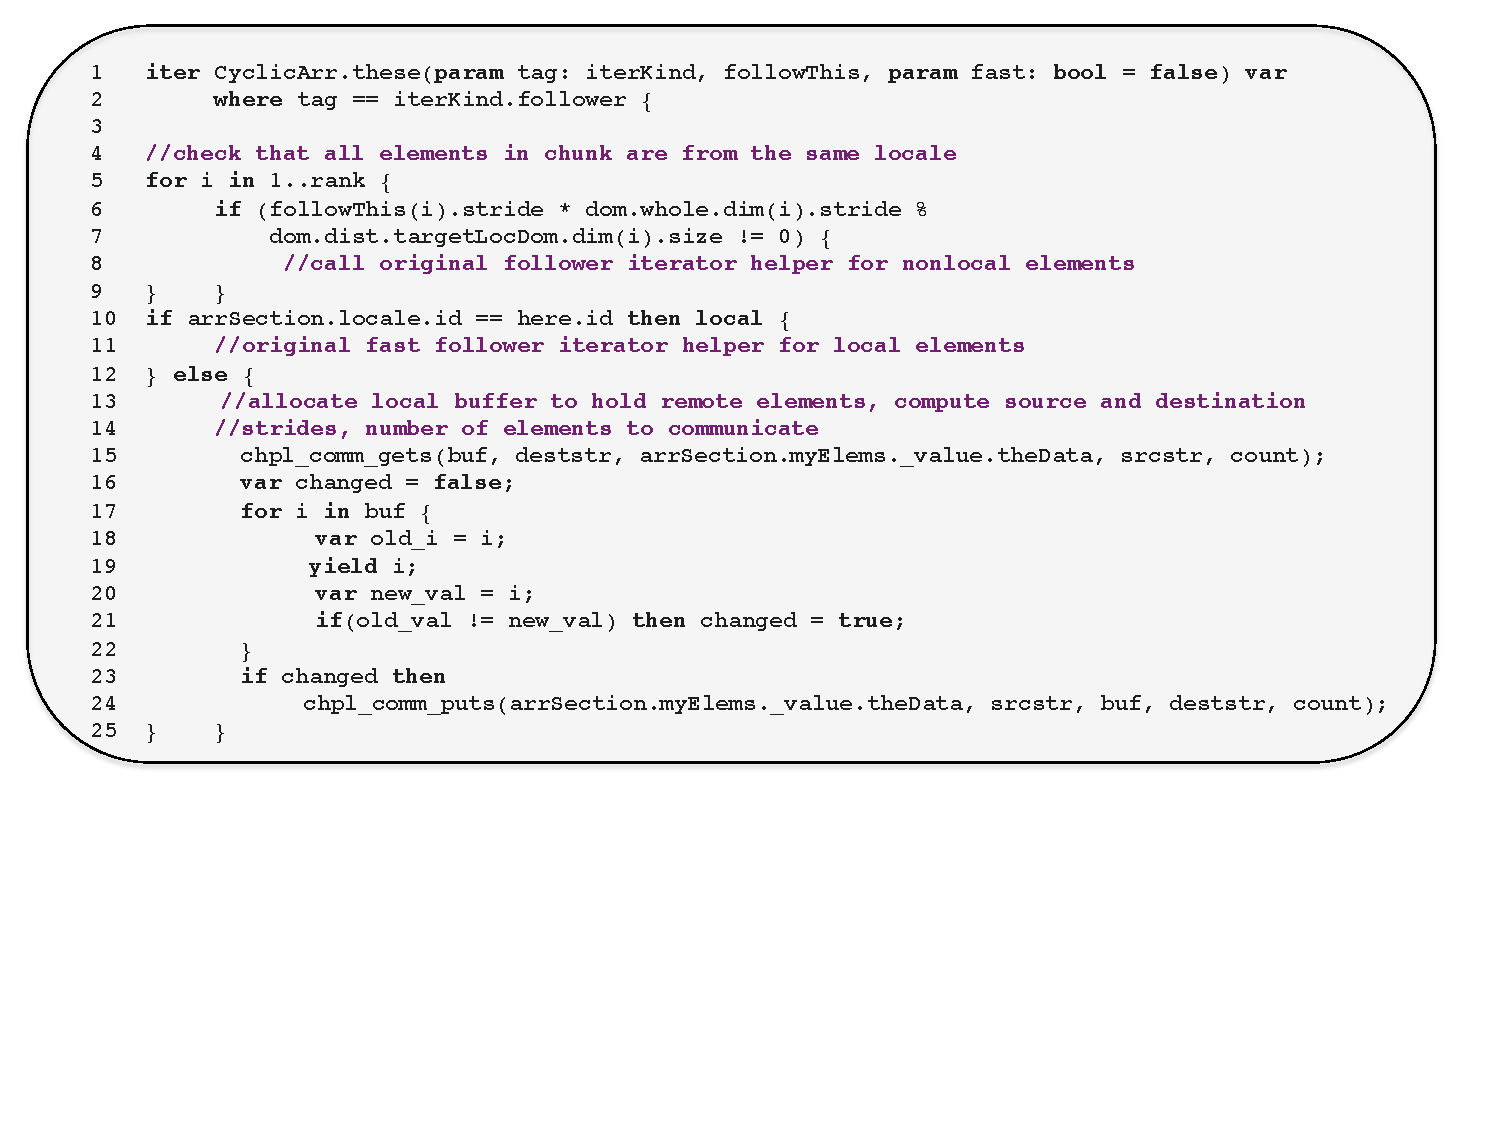
\includegraphics[scale=0.40]{./Figures/cyclic_muwu_follower}
	\caption{Cyclic with modulo unrolling WU caption}
	\label{cyclic_muwu_follower}
	\end{center}
\end{figure}

\subsection{Cyclic Distribution with Modulo Unrolling WU}\label{subsec:cyclic_modulo}

Modulo unrolling WU is implemented into the Chapel programming language through the Cyclic and Block Cyclic distribution modules, as opposed to being implemented via traditional compiler passes. This allows the optimization to be expressed using Chapel's higher-level language constructs, such as zippered iteration and array slicing. 

\begin{comment}
Modulo unrolling WU is implemented in the follower iterator of the Cyclic distribution. Based on the semantics of parallel zippered iteration, the leader iterator will divide up the iterations of the loop across the locales of the machine according to the first item in the zippering. This could mean that some portions of work will not be local to where the computation is taking place. The follower iterator in the Cyclic distribution recognizes whether or not its chunk of work is local or remote. If remote, all of the remote array elements are brought to the present locale in a local buffer using one \texttt{chpl\_comm\_gets} call. Finally, elements of the local buffer are now yielded back to the loop header. A loop body may modify the elements that are yielded to it via zippered iteration. To account for this, the follower iterator compares the element before it was yielded to the element after it was yielded. If any of the elements in the follower's chunk of work were modified, the entire local buffer is stored back to the remote local via one \texttt{chpl\_comm\_puts} call. 
\end{comment}

\subsection{Block Cyclic Distribution with Modulo Unrolling WU}\label{subsec:block_cyclic_modulo}

\begin{comment}
For the Chapel Block Cyclic implementation, both the leader and follower iterators have been modified to support the modulo unrolling WU optimization. Modulo unrolling, in its original form, is not compatible with the Block Cyclic distribution because consecutive array elements can reside on the same locale (this is defined by the block size parameter), which destroys the static locality information that we were able to use in the Cyclic distribution. The Block Cyclic leader iterator is now modified to choose slices of work such that the new "stride" is equal to the product of the block size and the cycle size. This way, when the work is passed to the follower iterator, elements that are in the same position within each block are guaranteed to be on the same locale. The follower iterator of the Block Cyclic distribution can now perform modulo unrolling WU in the same way as the Cyclic distribution. 
\end{comment}
%


\begin{figure}
	\begin{center}
	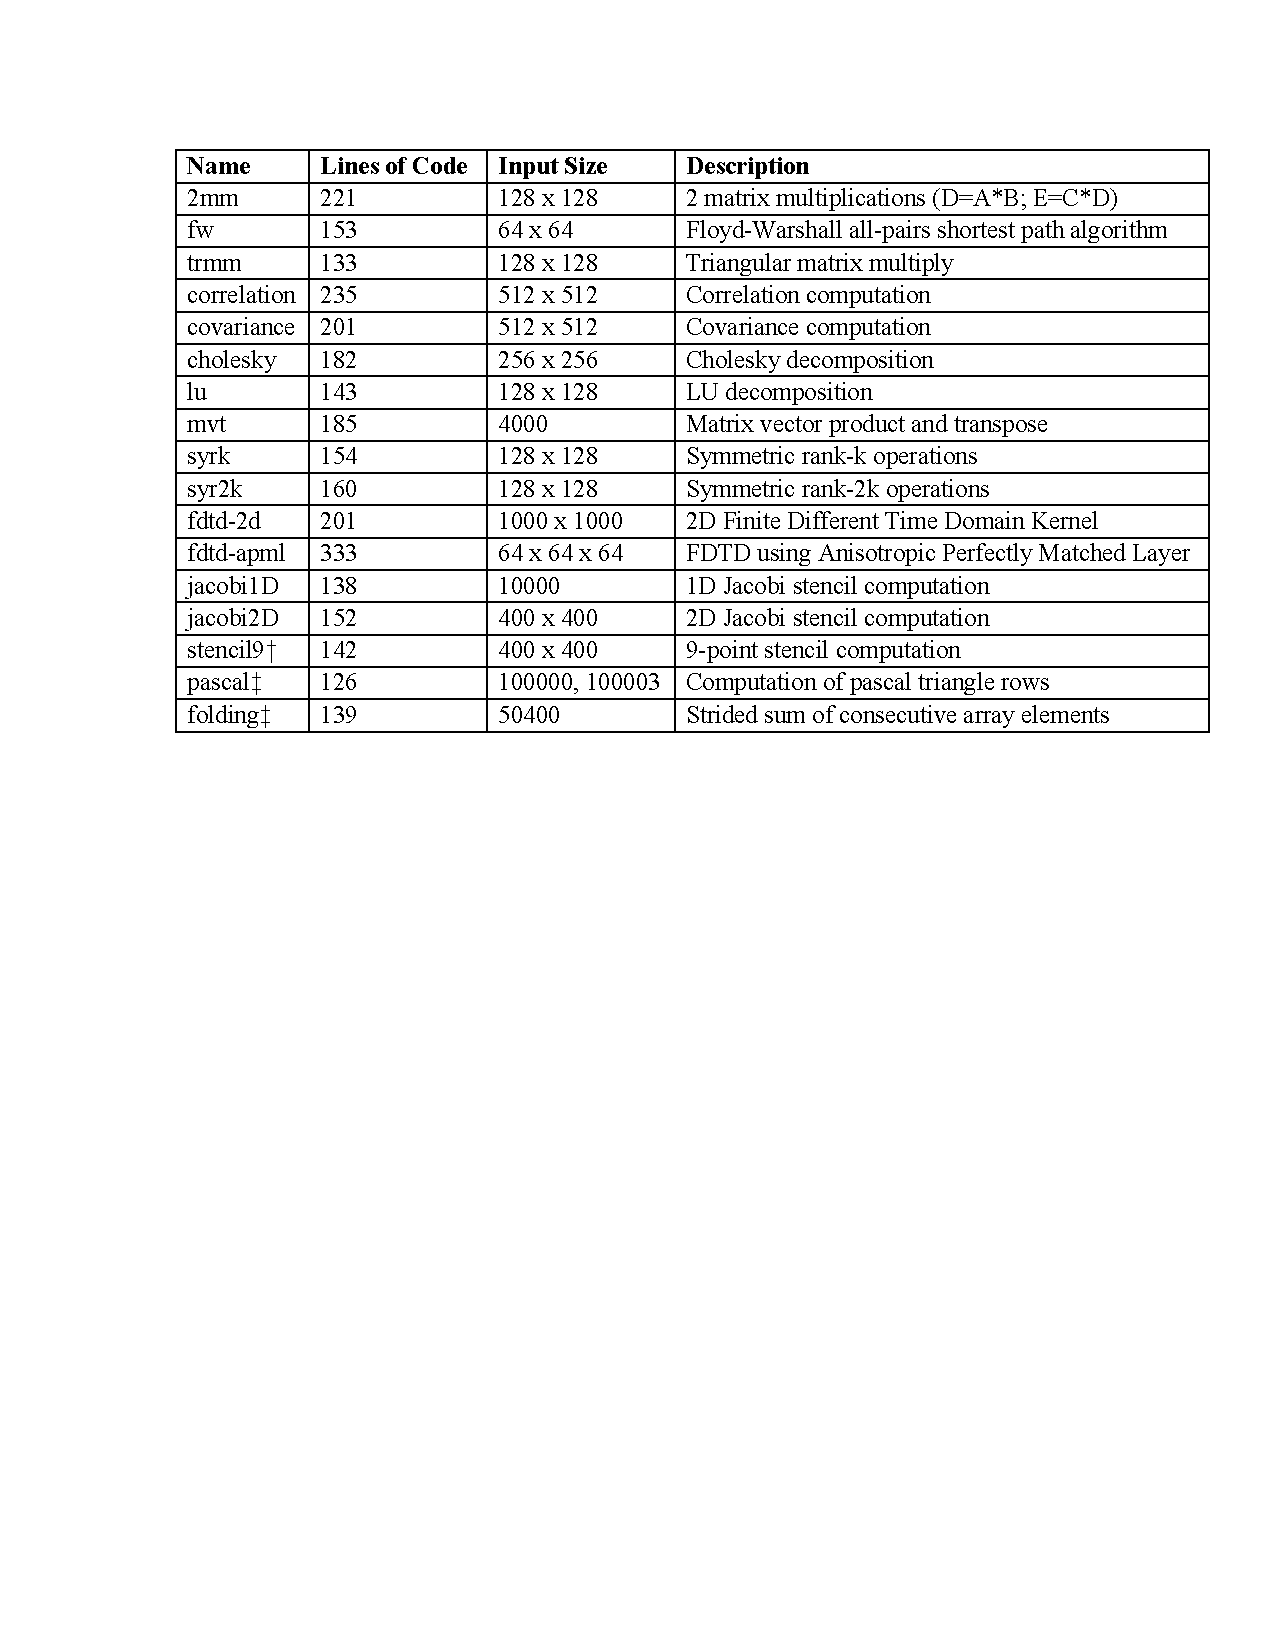
\includegraphics[scale=0.53]{./Figures/Benchmarks.pdf}
	\caption{Benchmark suite. Benchmarks with no symbol after their name were taken from the Polybench suite of benchmarks and translated to Chapel. Benchmarks with $\dagger$ are taken from the Chapel Trunk test directory. Benchmarks with $\ddagger$ were developed on our own in order to test specific data access patterns. }
	\label{benchmarks}
	\end{center}
\end{figure}

\section{Results}\label{sec:results}

To demonstrate the effectiveness of modulo unrolling WU in the Chapel Cyclic and Block Cyclic distributions, we present our results. We have composed a suite of seventeen parallel benchmarks shown in Figure \ref{benchmarks}. Each benchmark is written in Chapel and contains loops with affine array accesses that use zippered iterations, as discussed in \ref{sec:array_slicing}. Our suite of benchmarks contains programs with single, double, and triple nested affine loops. Additionally, our benchmark suite contains programs operating on one, two, and three-dimensional distributed arrays. Fourteen of the seventeen benchmarks are taken from the Polybench suite of benchmarks \cite{polybench} and are translated from C to Chapel by hand. The \textit{stencil9} benchmark was taken from the Chapel source trunk directory. The remaining two benchmarks, \textit{pascal} and \textit{folding}, were written by our group. \textit{pascal} is an additional benchmark other than \textit{jacobi1D} that is able to test Block Cyclic with modulo unrolling WU. \textit{folding} is the only benchmark in our suite that has strided affine array accesses. 

To evaluate improvements due to modulo unrolling WU, we run our benchmarks using the Cyclic and Block Cyclic distributions from the trunk revision 22919 of the Chapel compiler as well as the Cyclic and Block Cyclic distributions that have been modified to perform modulo unrolling WU, as described in Section \ref{sec:adaptation_in_chapel}. We measure both runtime and message count for each benchmark. We also compute the geometric means of all normalized runtimes and message count numbers for both distributions to get a sense on average of how much improvement modulo unrolling WU provided. 

When evaluating modulo unrolling WU used with the Block Cyclic distribution, we could only run two benchmarks out of our suite of seventeen because of limitations within the original Chapel Block Cyclic distribution. Many of our benchmarks operate on two or three-dimensional arrays and all require array slicing for the modulo unrolling WU optimization to apply. Both array slicing of multi-dimensional arrays and array slicing containing strides for one-dimensional arrays are not yet supported in the Chapel compiler's Block Cyclic distribution. Implementing such features remained outside the scope of this work. There was no limitation when evaluating modulo unrolling WU with the Cyclic distribution, and all seventeen benchmarks were tested. Once these missing features are implemented in the Chapel compiler, then our method will apply to all of our benchmarks.

\begin{figure}
	\begin{center}
	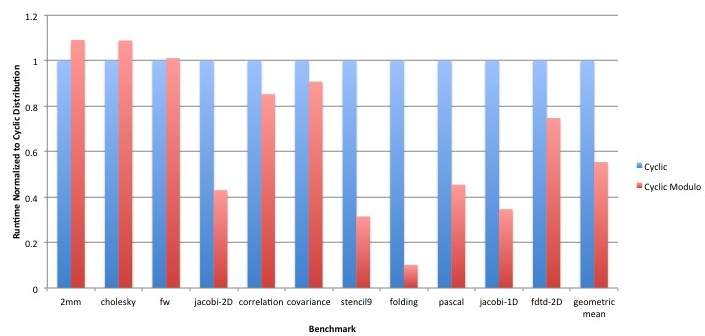
\includegraphics[scale=0.30]{./Figures/cyclic_runtime}
	\caption{Cyclic runtime.}
	\label{cyclic_runtime}
	\end{center}
\end{figure}

\begin{figure}
\begin{center}
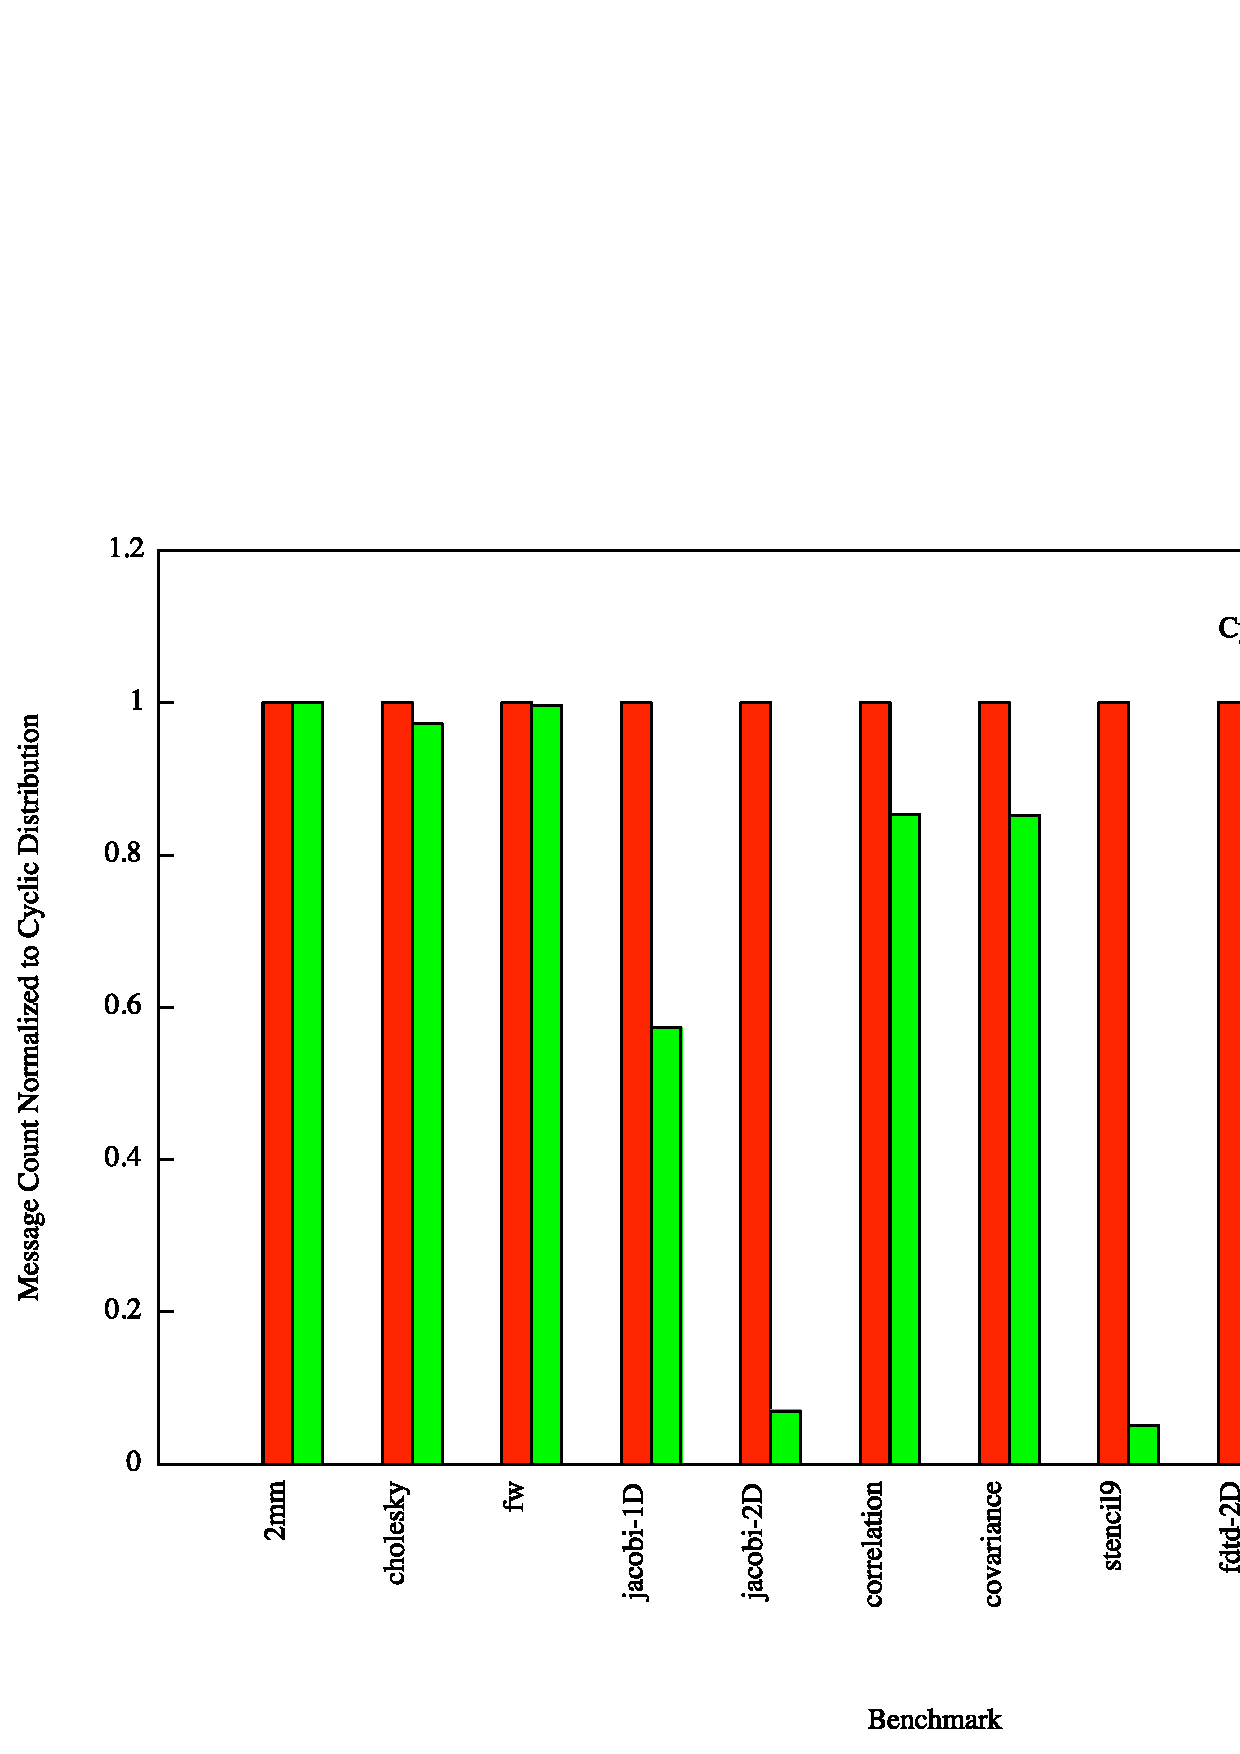
\includegraphics[scale=0.30]{./Figures/cyclic_message_count}
\caption{Cyclic message count.}
\label{cyclic_message_count}
\end{center}
\end{figure}

Figures \ref{cyclic_runtime} and \ref{cyclic_message_count} compare the normalized runtimes and message counts respectively for the Cyclic distribution and Cyclic distribution with modulo unrolling WU. For 8 of the 11 benchmarks, we see reductions in runtime when the modulo unrolling WU optimization is applied. On average, modulo unrolling WU results in a 45 percent decrease in runtime. For 9 of the 11 benchmarks, we see reductions in message counts when the modulo unrolling WU optimization is applied. On average, modulo unrolling WU results in 76 percent fewer messages. 

Some detailed observations on Figures \ref{cyclic_runtime} and \ref{cyclic_message_count} follow. Two of the benchmarks, \textit{cholesky} and \textit{fw}, showed slight improvements in message count when using modulo unrolling WU but did not show improvements in runtime. For the \textit{2mm} benchmark, both runtime and message count did not improve when using modulo unrolling WU. For these benchmarks, the ratio of the problem size to number of locales is not high enough, leading to an insufficient amount of aggregation possible for the computation to see performance improvements. An increase in the number of locales on a system leads to fewer data elements per locale, which naturally means fewer data elements can be aggregated. When this occurs, the cost of performing bulk transfers of a few data elements is more expensive than transferring elements individually. 

\begin{figure}
\begin{center}
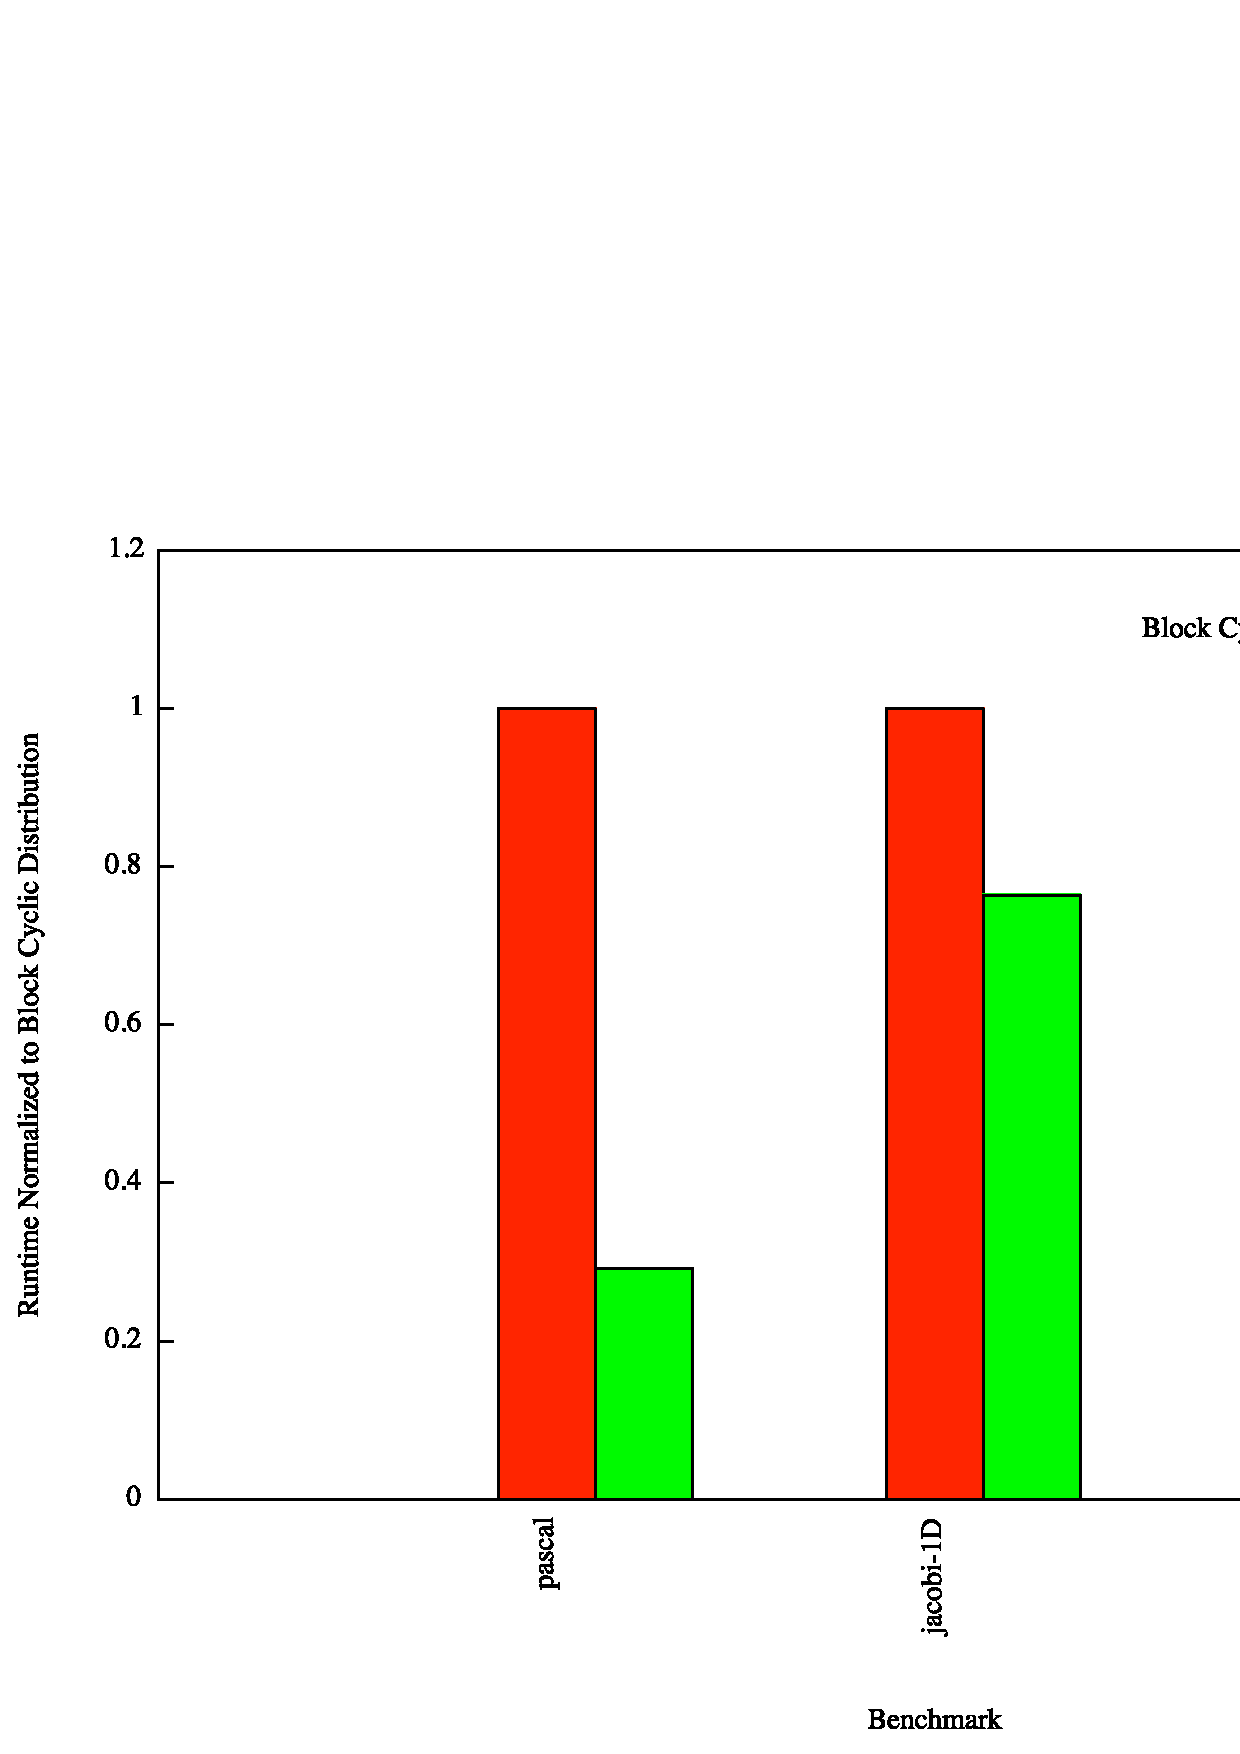
\includegraphics[scale=0.30]{./Figures/block_cyclic_runtime}
\caption{Block Cyclic runtime.}
\label{block_cyclic_runtime}
\end{center}
\end{figure}

\begin{figure}
\begin{center}
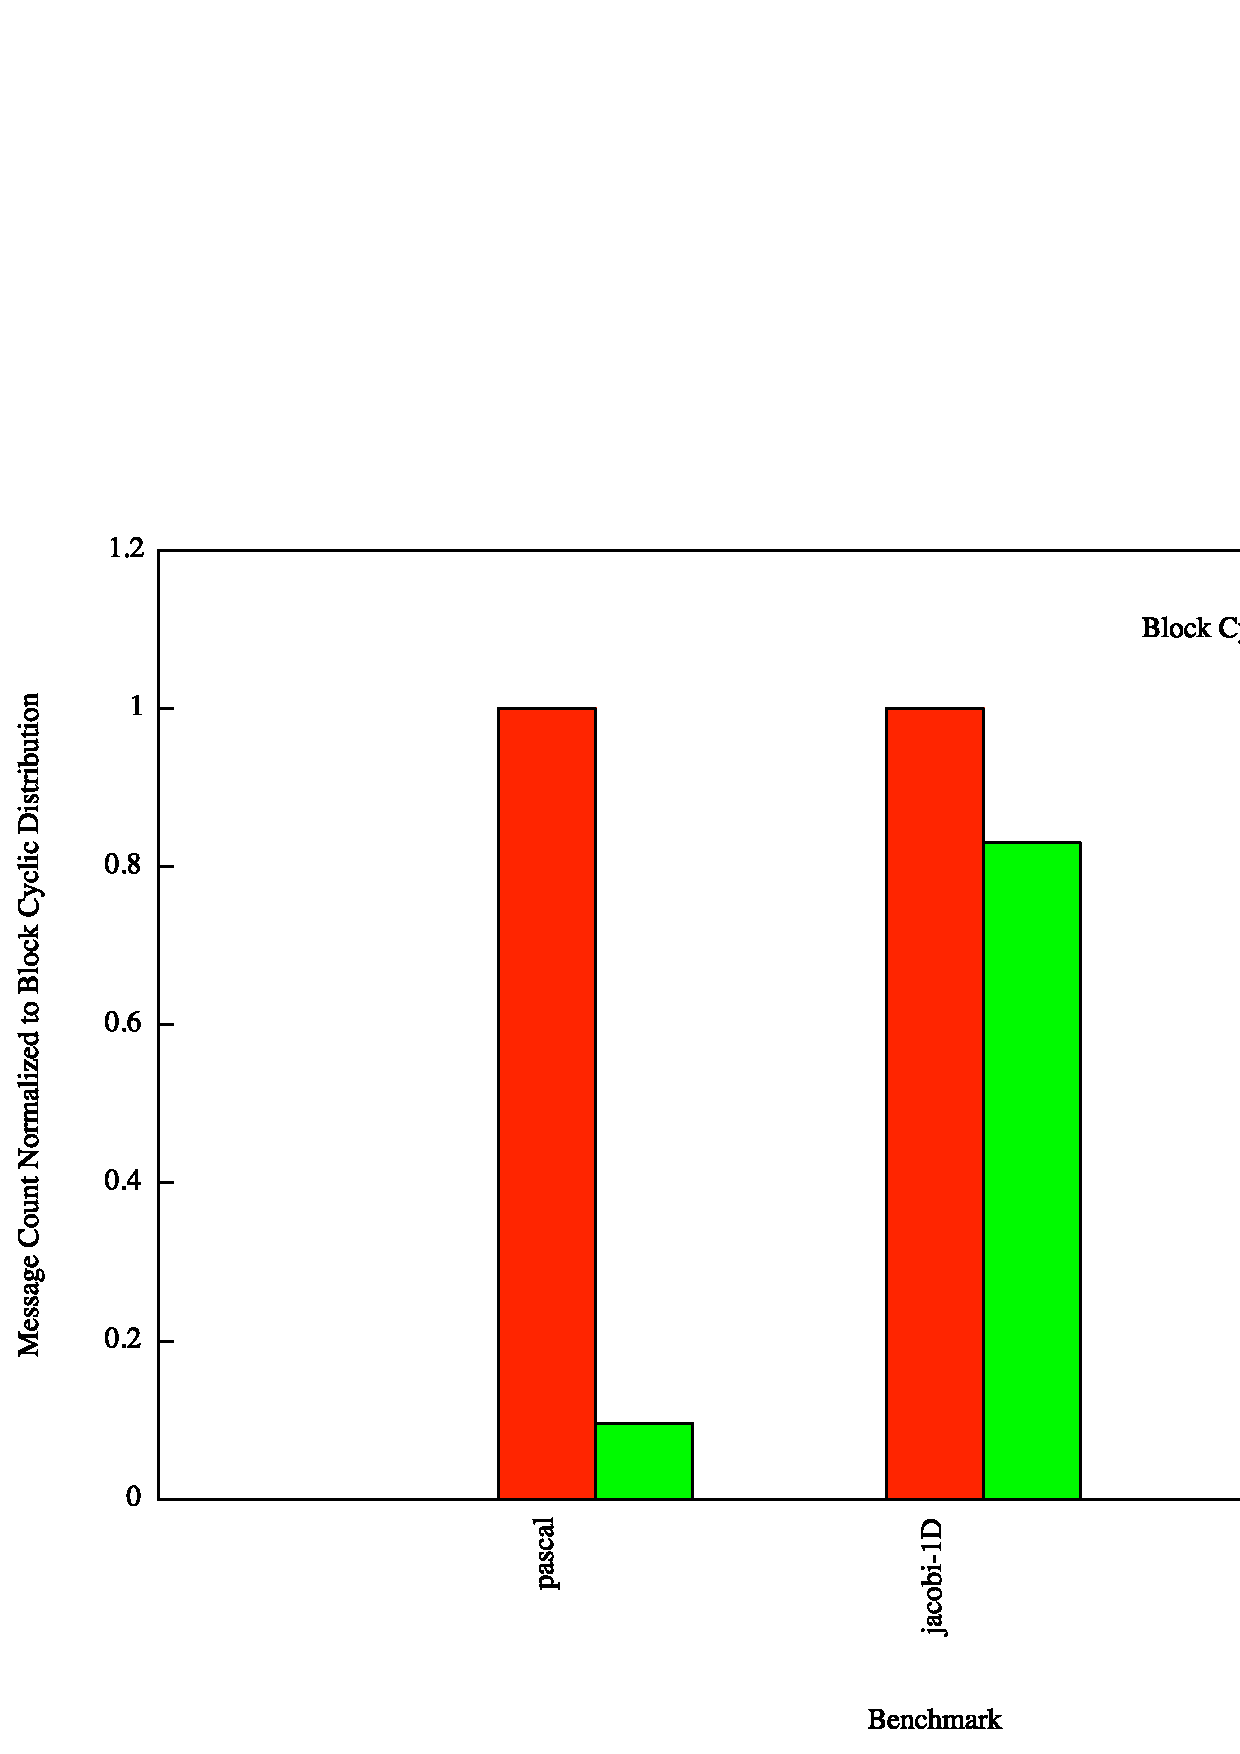
\includegraphics[scale=0.30]{./Figures/block_cyclic_message_count}
\caption{Block Cyclic message count.}
\label{block_cyclic_message_count}
\end{center}
\end{figure}

Figures \ref{block_cyclic_runtime} and \ref{block_cyclic_message_count} compare the normalized runtimes and message counts respectively for the Block Cyclic distribution and Block Cyclic distribution with modulo unrolling WU. For both benchmarks, we see reductions in runtime when the modulo unrolling WU optimization is applied. On average, modulo unrolling WU results in a 52 percent decrease in runtime. For both benchmarks, we see reductions in message counts when the modulo unrolling WU optimization is applied. On average, modulo unrolling WU results in 72 percent fewer messages. 
\section{Future Work}\label{sec:future_work}

As presented, the modulo unrolling WU optimization can be improved upon in a few ways to achieve even better performance in practice. First, there is currently no limit on the number of array elements that an aggregate message may contain. For applications with extremely large data sets, buffers containing remote data elements may become too large and exceed the memory budget of a particular locale. This may slow down other programs running on the system. A naive solution to this problem is to just turn off the optimization when the aggregate message is deemed too large and communicate remote data elements individually. A better solution would be to perform strip mining where the aggregate message is broken down into smaller aggregate messages of a configurable threshold size. 

The two forms of bulk communication used in this work (\texttt{chpl\_comm\_gets} and \texttt{chpl\_comm\_puts}) are both blocking communication calls. Our optimization might achieve better performance if it used a non-blocking strided bulk communication scheme. That way, communication and computation may be able to occur in parallel. 

Finally, it would be extremely beneficial if our implementation of modulo unrolling WU in the Cyclic follower iterator did not slow down programs with few data elements per chunk of parallel work. Ideally, these programs should, in the worst case, run as fast as they would if the original Chapel Cyclic follower iterator was used. Our research group is currently working on adding a dynamic check within the follower iterator that tests whether the number of data elements per chunk of parallel work is above the threshold where aggregation is still profitable. If not, the original follower iterator without modulo unrolling WU is called. 


%\section{Conclusion}\label{sec:conclusion} 



{
\begin{singlespace}
\vspace{-3ex}
\bibliography{bibliography}
\vspace{-2ex}
\bibliographystyle{ieeetr}
\end{singlespace}
}

\end{document}
